\documentclass[twocolumn,11pt,a4paper]{article}

%% -----------------------------------------------------------------------
%%  Packages
%% -----------------------------------------------------------------------
\usepackage{amsmath,amssymb,amsthm}
\usepackage{mathtools}
\usepackage{microtype}
\usepackage{geometry}
\geometry{a4paper, top=2.2cm, bottom=2.2cm, left=1.8cm, right=1.8cm, columnsep=0.7cm}
\usepackage{hyperref}
\hypersetup{colorlinks=true,linkcolor=blue,citecolor=blue,urlcolor=blue}
\usepackage{cleveref}
\usepackage{booktabs}
\usepackage{array}
\usepackage{enumitem}
\usepackage{xcolor}
\usepackage{natbib}
\bibpunct{[}{]}{,}{n}{}{;}
\usepackage{titlesec}
\usepackage{abstract}
\usepackage{graphicx}

%% -----------------------------------------------------------------------
%%  Theorem environments
%% -----------------------------------------------------------------------
\newtheorem{theorem}{Theorem}[section]
\newtheorem{lemma}[theorem]{Lemma}
\newtheorem{proposition}[theorem]{Proposition}
\newtheorem{corollary}[theorem]{Corollary}
\newtheorem{definition}[theorem]{Definition}
\newtheorem{construction}[theorem]{Construction}
\newtheorem{example}[theorem]{Example}
\theoremstyle{remark}
\newtheorem{remark}[theorem]{Remark}
\newtheorem{econinterp}[theorem]{Economic Interpretation}
\newtheorem{comparison}[theorem]{Comparison}

%% -----------------------------------------------------------------------
%%  Mathematical macros (inherited from companion papers)
%% -----------------------------------------------------------------------
\newcommand{\R}{\mathbb{R}}
\newcommand{\N}{\mathbb{N}}
\newcommand{\Sflat}{S_{\flat}}
\newcommand{\Sig}{\Sigma}
\newcommand{\Ksp}{\mathcal{K}}
\newcommand{\Rec}{\mathcal{R}}
\newcommand{\Meth}{\mathcal{M}}
\newcommand{\Goal}{\mathcal{G}}
\newcommand{\Act}{\mathrm{Act}}
\newcommand{\Reach}{\mathrm{Reach}}
\newcommand{\tol}{\tau}
\newcommand{\Ens}{\mathcal{E}}
\newcommand{\Compose}{\diamond}

%% -----------------------------------------------------------------------
%%  New macros (this paper)
%% -----------------------------------------------------------------------
\newcommand{\srad}{\rho}                  % spectral radius of contraction
\newcommand{\sgap}{\delta}                % spectral gap
\newcommand{\ClassE}{\mathcal{C}_E}       % Borel-Cantelli efficiency class
\newcommand{\ClassO}{\mathcal{C}_\Omega}  % omega-inefficiency class
\newcommand{\logfl}{\ell}                 % log-floor of a single agent
\newcommand{\Logfl}{L}                    % cumulative log-floor
\newcommand{\geomean}{\hat{\beta}}        % geometric mean of floors
\newcommand{\Var}{\mathrm{Var}}           % variance operator
\newcommand{\CV}{\sigma_r}               % coefficient of variation
\newcommand{\Crit}{\beta_{\mathrm{c}}}   % critical floor threshold
\newcommand{\Sflathom}{S_{\flat,\mathrm{hom}}}  % homogeneous-ensemble floor

%% -----------------------------------------------------------------------
%%  Title block
%% -----------------------------------------------------------------------
\title{\textbf{The Heterogeneity Theorem for Market Information:\\
Infinite Ensembles, Spectral Theory of the Purpose Functional,\\
and Universality Classes of Market Efficiency}}

\author{Kundai Farai Sachikonye\\[4pt]
\small Technical University of Munich\\
\small AIMe Registry for Artificial Intelligence\\
\small Maximus-von-Imhof-Forum 3, 85354 Freising, Germany\\
\small \texttt{kundai.sachikonye@wzw.tum.de}}

\date{}

\begin{document}

\maketitle

%% -----------------------------------------------------------------------
%%  Abstract
%% -----------------------------------------------------------------------
\begin{abstract}
\noindent
This paper proves the Heterogeneity Theorem for market information and
completes the mathematical theory of bounded economic agents with three
principal extensions: infinite ensembles, the spectral theory of the purpose
functional, and the classification of markets into universality classes.
Taking the agent triple $(R,M,G)$, composite floor
$\Sflat(\Ens_n) = \prod_{i=1}^n \Sflat(A_i)/\Sigma^{n-1}$, and
purpose-cell contraction from the companion
papers~\cite{sachikonye2025agents,sachikonye2025market} as primitives, we
prove ten principal results:
(i)~the \emph{Heterogeneity Dominance Theorem} --- the composite floor is a
Schur-concave function of the floor vector, so greater heterogeneity
(majorization) strictly reduces the composite floor at any fixed arithmetic
mean;
(ii)~the \emph{Borel--Cantelli Classification} --- every infinite ensemble
belongs to exactly one of two universality classes, $\ClassE$ (efficient,
$\Sflat(\Ens_n)\to 0$) or $\ClassO$ (omega-inefficient, $\Sflat(\Ens_n)>0$),
separated by the convergence of $\sum_i \log(\Sigma/\Sflat(A_i))$;
(iii)~the \emph{Spectral Gap Theorem} --- the purpose-cell contraction has
spectral radius $\srad_\Ens = \Sflat(\Ens)/\Sigma$ and spectral gap
$\sgap_\Ens = 1 - \srad_\Ens$, which is strictly increasing in
heterogeneity;
(iv)~the \emph{Heterogeneity Theorem} --- among all $n$-agent ensembles with
fixed arithmetic mean floor, the most heterogeneous ensemble minimises
$\srad_\Ens$ and maximises $\sgap_\Ens$;
(v)~the \emph{Information Aggregation Rate Theorem} --- log-floors are
additive: $\log(\Sigma/\Sflat(\Ens_n)) = \sum_{i=1}^n \logfl_i$ where
$\logfl_i = \log(\Sigma/\Sflat(A_i))$ is the marginal information
contribution of agent $i$;
(vi)~the \emph{Optimal Recruitment Theorem} --- the cumulative composite
floor is minimised when agents join in ascending floor order, by the
rearrangement inequality;
(vii)~the \emph{Phase Transition Theorem} --- the transition from Class
$\ClassO$ to Class $\ClassE$ is sharp at zero informed participation
($p_c=0$): any positive fraction of bounded agents guarantees eventual
efficiency;
(viii)~the \emph{Floor-Variance Efficiency Bound} ---
$\Sflat(\Ens_n) \le (\bar{\beta}/\Sigma)^n \Sigma\,
e^{-n\CV^2/2+O(n\CV^3)}$, where $\CV = \Var(\beta_i)^{1/2}/\bar\beta$;
(ix)~the \emph{Stability of Efficiency Class} --- both $\ClassE$ and
$\ClassO$ are invariant under replacement of any finite sub-ensemble;
and
(x)~the \emph{Critical Floor Theorem} --- the critical floor
$\Crit = \Sigma/e$ separates agents whose marginal contribution exceeds one
nat from those whose contribution falls below one nat; no finite ensemble
of agents with $\beta_i \ge \Crit$ can achieve sub-$1/e$ composite
normalisation.
Forty-five numerical experiments verify all claims to machine precision
(maximum relative error $< 10^{-14}$).
\end{abstract}

\tableofcontents

\bigskip

%% ======================================================================
\section{Introduction}
\label{sec:intro}
%% ======================================================================

\subsection{The Efficiency Question}
\label{sec:intro:eff}

Papers~1 and~2 of this series established that bounded agents can reach
equilibrium without convexity, common knowledge, or rational expectations.
Paper~1~\cite{sachikonye2025agents} derived the receiver $(K,D,\Pi,\beta)$
and proved that the floor $\beta>0$ is irreducible.  Paper~2~\cite{sachikonye2025market}
proved that ensembles of heterogeneous bounded agents converge to a purpose
cell $C^*$ and characterised the composite floor
$\Sflat(\Ens_n) = \prod_{i=1}^n \Sflat(A_i)/\Sigma^{n-1}$ as the binding
constraint on market information efficiency.

The question left open is: \emph{what drives the rate at which the composite
floor decays toward zero}?  The Borel--Cantelli condition of Paper~2
($\sum_i \log(1/q_i) = \infty$ where $q_i = \Sflat(A_i)/\Sigma$) gives
the qualitative criterion for eventual efficiency.  But it does not
distinguish the rate of approach, it does not identify the optimal ensemble
structure, and it does not classify the universality classes of market
efficiency.

\medskip
\noindent\textbf{Classical efficiency concepts and their limits.}
The Efficient Market Hypothesis~\cite{fama1970} states that prices fully
reflect all available information.  Grossman and Stiglitz~\cite{grossmanstiglitz1980}
proved this impossible at finite cost: if markets were perfectly efficient,
no agent would spend resources gathering information.  The resolution is that
real markets achieve a \emph{partially efficient} equilibrium
$\Sflat(\Ens_n) > 0$ that approaches full efficiency $\Sflat(\Ens_\infty)=0$
only asymptotically.  The present paper characterises precisely how this
asymptotic approach depends on the heterogeneity of agents.

Shannon's information theory~\cite{shannon1948} suggests that diverse sources
yield more information than redundant ones.  The wisdom-of-crowds
literature~\cite{surowiecki2004} documents empirically that heterogeneous
crowds outperform homogeneous ones.  The present paper proves these
observations as theorems in the receiver-agent framework, deriving the
precise rate advantage of heterogeneity.

\subsection{Main Contributions}
\label{sec:intro:contrib}

\begin{enumerate}[leftmargin=*, label=\textbf{(\roman*)}]
\item \textbf{Heterogeneity Dominance Theorem}
  (\cref{thm:dominance}).
  The composite floor $\Sflat(\Ens_n)$ is a Schur-concave function of
  $(\Sflat(A_1),\ldots,\Sflat(A_n))$.  If ensemble $\Ens$ is more
  heterogeneous than $\Ens'$ in the majorization order, then
  $\Sflat(\Ens) \le \Sflat(\Ens')$.

\item \textbf{Borel--Cantelli Classification}
  (\cref{thm:bc-classification}).
  Every infinite ensemble $\Ens_\infty$ belongs to exactly one of two
  universality classes.  Class $\ClassE$ (efficient): $\sum_i \logfl_i =
  +\infty$, $\Sflat(\Ens_n) \to 0$.  Class $\ClassO$ (omega-inefficient):
  $\sum_i \logfl_i < +\infty$, $\Sflat(\Ens_n) \to \Sflat(\Ens_\infty)>0$.

\item \textbf{Spectral Gap Theorem}
  (\cref{thm:spectral-gap}).
  The purpose-cell contraction $\Psi_\Ens$ has spectral radius
  $\srad_\Ens = \Sflat(\Ens)/\Sigma \in (0,1)$ and spectral gap
  $\sgap_\Ens = 1 - \srad_\Ens$.  The purpose flow converges at rate
  $\kappa_\Ens^t$ and perturbations of magnitude $\varepsilon$ to
  $\Sflat(\Ens)$ shift the equilibrium cell by at most
  $\varepsilon/\sgap_\Ens$ in Hausdorff distance.

\item \textbf{Heterogeneity Theorem}
  (\cref{thm:heterogeneity}).
  Among all $n$-agent ensembles with arithmetic mean floor $\bar\beta$,
  the most heterogeneous ensemble (in the majorization order) achieves the
  strictly smallest $\srad_\Ens$ and strictly largest $\sgap_\Ens$.
  Homogeneous ensembles (all $\beta_i = \bar\beta$) are the unique maximisers
  of $\srad_\Ens$ at fixed mean.

\item \textbf{Information Aggregation Rate Theorem}
  (\cref{thm:rate}).
  For any ensemble $\Ens_n = (A_1,\ldots,A_n)$,
  $\log(\Sigma/\Sflat(\Ens_n)) = \sum_{i=1}^n \logfl_i$ where
  $\logfl_i = \log(\Sigma/\Sflat(A_i)) > 0$ is the \emph{log-floor} of
  agent $i$.  The log-floors are exactly additive: each new agent
  contributes $\logfl_{n+1}$ independently of the current ensemble size.

\item \textbf{Optimal Recruitment Theorem}
  (\cref{thm:recruitment}).
  For a fixed multiset of agent floors, the cumulative composite floor
  $\prod_{k=1}^n \Sflat(\Ens_k)$ — which measures total information cost
  over all $n$ recruitment steps — is minimised by recruiting in ascending
  floor order (best agents first).  Any other order incurs strictly higher
  cumulative cost.

\item \textbf{Phase Transition Theorem}
  (\cref{thm:phase}).
  Consider an infinite market where a fraction $p$ of agents have bounded
  floor $\beta_L < \Sigma$ and the remainder are uninformed with
  $\beta_H \to \Sigma^-$.  The transition from Class $\ClassO$ to Class
  $\ClassE$ is sharp at $p_c = 0$: any positive informed participation
  $p>0$ places the market in Class $\ClassE$.  The convergence rate exponent
  is linear in $p$: $\Sflat(\Ens_n) \approx (\beta_L/\Sigma)^{pn}$ for
  large $n$.

\item \textbf{Floor-Variance Efficiency Bound}
  (\cref{thm:fvb}).
  Let $\bar\beta$ be the arithmetic mean floor and $\CV = \Var(\beta_i)^{1/2}/
  \bar\beta$ the coefficient of variation.  Then
  $\Sflat(\Ens_n) \le (\bar\beta^n/\Sigma^{n-1}) \cdot
  e^{-n\CV^2/2 + O(n\CV^3)}$, with equality iff all $\beta_i$ are equal.
  Heterogeneity saves a factor of $e^{-n\CV^2/2}$ relative to a
  homogeneous ensemble of the same mean.

\item \textbf{Stability of Efficiency Class}
  (\cref{thm:stability}).
  Both $\ClassE$ and $\ClassO$ are invariant under replacement of any finite
  sub-ensemble.  No finite perturbation can move an infinite ensemble between
  classes.

\item \textbf{Critical Floor Theorem}
  (\cref{thm:critical}).
  The critical floor $\Crit = \Sigma/e$ is the unique threshold at which an
  agent's log-floor contribution equals exactly one nat.  Agents with
  $\beta_i < \Crit$ contribute more than one nat; agents with
  $\beta_i > \Crit$ contribute less.  No ensemble composed entirely of agents
  with $\beta_i \ge \Crit$ can achieve $\Sflat(\Ens_n) < e^{-n}\Sigma$.
\end{enumerate}

\subsection{Organization}
\label{sec:intro:org}

\Cref{sec:prelim} recaps the inherited framework.
\Cref{sec:infinite} defines infinite ensembles and limit floors.
\Cref{sec:spectral} develops the spectral theory.
\Cref{sec:dominance} proves Heterogeneity Dominance.
\Cref{sec:classes} establishes the Borel--Cantelli classification.
\Cref{sec:heterogeneity} proves the Heterogeneity Theorem.
\Cref{sec:rate} establishes the Information Aggregation Rate and Optimal
Recruitment Theorem.
\Cref{sec:fvb} proves the Floor-Variance Efficiency Bound and Phase
Transition Theorem.
\Cref{sec:stability} proves Stability of Efficiency Class and the Critical
Floor Theorem.
\Cref{sec:numerical} presents forty-five numerical experiments.
\Cref{sec:literature} surveys connections to the literature.
\Cref{sec:conclusion} states conclusions.

%% ======================================================================
\section{Inherited Framework}
\label{sec:prelim}
%% ======================================================================

We summarise the primitives established in the companion
papers~\cite{sachikonye2025agents,sachikonye2025market}; all proofs are
deferred to those works.

A \emph{receiver} is a four-tuple $\Rec = (K,D,\Pi,\beta)$ with $K$ the
knowledge framework, $D: X \to K$ the decoder, $\Pi: K \to 2^X$ the
candidate-projection, and $\beta > 0$ the irreducible receiver floor.  The
S-functional at state $x$ targeting cell $C \subseteq X$ is
$S(\Rec,x;C) = \inf_{c\in\Pi(D(x))} d(c,C) + \beta$.

An \emph{agent triple} is $A = (\Rec,\Meth,\Goal)$ with methodology
$\Meth$ and goal set $\Goal$.  The agent floor is
$\Sflat(A) = \beta \cdot \Sflat(\Meth)/\Sigma$, where
$\Sflat(\Meth) = \sigma\kappa/(1-\kappa)$ is the Banach fixed point of the
methodology contraction~\cite{sachikonye2025agents}.

A finite \emph{ensemble} $\Ens_n = (A_1,\ldots,A_n)$ has composite floor
\begin{equation}
  \Sflat(\Ens_n) \;=\; \frac{\prod_{i=1}^n \Sflat(A_i)}{\Sigma^{n-1}}
  \label{eq:composite-floor}
\end{equation}
and multi-agent S-functional
$S(\Ens_n,x;C) = \min_{1\le i\le n} S(A_i,x;C)$~\cite{sachikonye2025market}.

Throughout this paper $\Sigma > 0$ is the maximal semantic distance
(canonical value $\Sigma = 100$), and $q_i = \Sflat(A_i)/\Sigma \in (0,1)$
is the \emph{normalised floor} of agent $i$.  We write
$\boldsymbol\beta = (\beta_1,\ldots,\beta_n)$ for the floor vector of a
finite ensemble, ordered so that $\beta_{(1)} \le \cdots \le \beta_{(n)}$
are the order statistics.

%% ======================================================================
\section{Infinite Ensembles and the Limit Floor}
\label{sec:infinite}
%% ======================================================================

\begin{definition}[Infinite ensemble]
\label{def:infinite-ens}
An \emph{infinite ensemble} is a countably infinite sequence
$\Ens_\infty = (A_1, A_2, \ldots)$ of agent triples, each with positive
individual floor $\Sflat(A_i) > 0$.  The truncation to the first $n$ agents
is $\Ens_n = (A_1,\ldots,A_n)$.
\end{definition}

\begin{proposition}[Floor monotonicity]
\label{prop:monotone}
For any infinite ensemble $\Ens_\infty$, the composite floor sequence
$\{\Sflat(\Ens_n)\}_{n\ge 1}$ is strictly decreasing:
$\Sflat(\Ens_{n+1}) = \Sflat(\Ens_n) \cdot q_{n+1} < \Sflat(\Ens_n)$.
\end{proposition}
\begin{proof}
From~\eqref{eq:composite-floor},
$\Sflat(\Ens_{n+1}) = \prod_{i=1}^{n+1}\Sflat(A_i)/\Sigma^n =
\Sflat(\Ens_n) \cdot \Sflat(A_{n+1})/\Sigma = \Sflat(\Ens_n) \cdot q_{n+1}$.
Since $q_{n+1} \in (0,1)$, the sequence is strictly decreasing.
\end{proof}

\begin{proposition}[Limit floor existence]
\label{prop:limit}
The sequence $\{\Sflat(\Ens_n)\}_{n\ge 1}$ is bounded below by $0$ and
strictly decreasing, so the limit
$\Sflat(\Ens_\infty) := \lim_{n\to\infty} \Sflat(\Ens_n) \ge 0$
exists.  In normalised form, $\Sflat(\Ens_\infty)/\Sigma = \prod_{i=1}^\infty q_i
\in [0,1)$.
\end{proposition}
\begin{proof}
Strict decrease and lower boundedness yield existence by the monotone
convergence theorem.  The limit equals $\Sigma\prod_{i=1}^\infty q_i$ because
$\Sflat(\Ens_n)/\Sigma = \prod_{i=1}^n q_i$, a partial product of numbers
in $(0,1)$, which converges to its infinite product in $[0,1)$.
\end{proof}

\begin{remark}
The infinite product $\prod_{i=1}^\infty q_i$ lies in $(0,1)$ if and only if
$\sum_{i=1}^\infty (1-q_i) < \infty$.  This is the classical criterion for
convergence of an infinite product of positive terms.  Its relationship to
the Borel--Cantelli condition is the subject of \cref{sec:classes}.
\end{remark}

%% ======================================================================
\section{Spectral Theory of the Purpose Functional}
\label{sec:spectral}
%% ======================================================================

\subsection{The Purpose-Cell Contraction}
\label{sec:spectral:contraction}

The purpose-cell contraction $\Psi_\Ens$ was established in
Paper~2~\cite{sachikonye2025market}.  We restate its key property here for
spectral analysis.

Let $(\mathrm{Cell}(X), d_H)$ denote the space of closed bounded subsets of $X$
equipped with the Hausdorff metric $d_H$.  The \emph{purpose functional} of
ensemble $\Ens$ is
\[
  \Phi_\Ens(C) \;:=\; \sup_{x \in X} S(\Ens, x; C)
  \;=\; \Sflat(\Ens) + \tol(C),
\]
where $\tol(C)$ is the cell tolerance.  The \emph{purpose-cell contraction}
$\Psi_\Ens: \mathrm{Cell}(X) \to \mathrm{Cell}(X)$ is the map that sends $C$
to the maximal cell $C'$ satisfying $\Phi_\Ens(C') = \Sflat(\Ens)$.  By
the Banach fixed-point theorem~\cite{sachikonye2025market}, $\Psi_\Ens$
has a unique fixed point $C^* \in \mathrm{Cell}(X)$, the \emph{purpose cell}
or \emph{market equilibrium cell}.

\begin{definition}[Spectral radius of the contraction]
\label{def:spectral-radius}
The \emph{spectral radius} of $\Psi_\Ens$ is the Lipschitz constant of
$\Psi_\Ens$ on $(\mathrm{Cell}(X), d_H)$:
\[
  \srad_\Ens \;:=\; \mathrm{Lip}(\Psi_\Ens)
  \;=\; \frac{\Sflat(\Ens)}{\Sigma} \;\in\; (0,1).
\]
\end{definition}

\begin{definition}[Spectral gap]
\label{def:spectral-gap}
The \emph{spectral gap} of $\Psi_\Ens$ is
\[
  \sgap_\Ens \;:=\; 1 - \srad_\Ens \;=\; 1 - \frac{\Sflat(\Ens)}{\Sigma}
  \;\in\; (0,1).
\]
\end{definition}

\subsection{The Spectral Gap Theorem}
\label{sec:spectral:gap-thm}

\begin{theorem}[Spectral Gap]
\label{thm:spectral-gap}
Let $\Ens = (A_1,\ldots,A_n)$ be a finite ensemble with composite floor
$\Sflat(\Ens)$ and let $C^*$ be its purpose cell.  Then:
\begin{enumerate}[label=\textup{(\alph*)}]
\item \textbf{Convergence rate.}  For any initial cell $C_0 \in
  \mathrm{Cell}(X)$ in the reachability set,
  $d_H(\Psi_\Ens^t(C_0), C^*) \le \srad_\Ens^t \cdot d_H(C_0, C^*)$.
\item \textbf{Perturbation bound.}  If $\Sflat(\Ens)$ is perturbed by
  $\varepsilon > 0$ (e.g.\ by adding agents or altering floors), the
  equilibrium cell shifts by at most $\varepsilon/\sgap_\Ens$ in $d_H$.
\item \textbf{Heterogeneity monotonicity.}  $\sgap_\Ens$ is strictly
  increasing in the heterogeneity of the floor vector $\boldsymbol\beta$,
  at fixed arithmetic mean $\bar\beta$.
\end{enumerate}
\end{theorem}
\begin{proof}
\textit{(a)}  Since $\Psi_\Ens$ is a contraction with Lipschitz constant
$\srad_\Ens$, the standard Banach contraction estimate gives
$d_H(\Psi_\Ens^t(C_0), C^*) \le \srad_\Ens^t \cdot d_H(C_0, C^*)$.

\textit{(b)}  A perturbation $\varepsilon$ to $\Sflat(\Ens)$ changes
$\srad_\Ens$ by $\varepsilon/\Sigma$.  By a standard perturbation lemma for
contractive fixed points, the fixed point $C^*$ shifts by at most
$\varepsilon/(\Sigma(1-\srad_\Ens)) = \varepsilon/(\Sigma\sgap_\Ens)$.
Since $d_H$ is normalised so that $\Sigma = \mathrm{diam}(X)$, this equals
$\varepsilon/\sgap_\Ens$.

\textit{(c)}  By the Heterogeneity Dominance Theorem (\cref{thm:dominance}),
greater heterogeneity (in the majorization order) reduces $\Sflat(\Ens)$,
hence reduces $\srad_\Ens = \Sflat(\Ens)/\Sigma$ and increases
$\sgap_\Ens = 1 - \srad_\Ens$.
\end{proof}

\begin{econinterp}
\label{ei:spectral-gap}
The spectral gap $\sgap_\Ens$ is the market's \emph{information efficiency
coefficient}.  A large gap ($\sgap_\Ens \to 1$) means the composite floor
is near zero: the ensemble aggregates information almost perfectly and the
equilibrium cell is reached quickly from any initial condition.  A small gap
($\sgap_\Ens \to 0$) means the composite floor nearly equals $\Sigma$:
the market is almost completely informationally opaque and perturbations
to the equilibrium cell are amplified rather than damped.  Heterogeneity
increases $\sgap_\Ens$ because diverse information sources reduce the
composite floor faster than redundant ones.
\end{econinterp}

%% ======================================================================
\section{Heterogeneity Dominance}
\label{sec:dominance}
%% ======================================================================

\subsection{Majorization and Schur-Concavity}
\label{sec:dominance:schur}

\begin{definition}[Majorization]
\label{def:majorization}
For vectors $\boldsymbol\alpha, \boldsymbol\alpha' \in \R_{>0}^n$, we say
$\boldsymbol\alpha$ \emph{majorizes} $\boldsymbol\alpha'$ (written
$\boldsymbol\alpha \succ \boldsymbol\alpha'$) if, letting $\alpha_{(1)} \ge
\cdots \ge \alpha_{(n)}$ denote order statistics,
\[
  \sum_{i=1}^k \alpha_{(i)} \ge \sum_{i=1}^k \alpha_{(i)}'
  \quad \forall k = 1,\ldots,n-1,
  \qquad \text{and} \qquad
  \sum_{i=1}^n \alpha_i = \sum_{i=1}^n \alpha_i'.
\]
$\boldsymbol\alpha \succ \boldsymbol\alpha'$ means $\boldsymbol\alpha$ is
\emph{more spread out} than $\boldsymbol\alpha'$ with the same total.
\end{definition}

\begin{definition}[Schur-concavity]
\label{def:schur-concave}
A symmetric function $f: \R_{>0}^n \to \R$ is \emph{Schur-concave} if
$\boldsymbol\alpha \succ \boldsymbol\alpha'$ implies
$f(\boldsymbol\alpha) \le f(\boldsymbol\alpha')$.
\end{definition}

\begin{lemma}[Schur-Ostrowski criterion]
\label{lem:schur-ostrowski}
A differentiable symmetric function $f: \R_{>0}^n \to \R$ is Schur-concave
if and only if for all $i \neq j$ and all
$\boldsymbol\alpha \in \R_{>0}^n$,
\[
  (\alpha_i - \alpha_j)\!\left(\frac{\partial f}{\partial \alpha_i}
  - \frac{\partial f}{\partial \alpha_j}\right) \le 0.
\]
\end{lemma}
\begin{proof}
This is the classical Schur--Ostrowski characterisation of Schur-concave
functions; see~\cite{marshall2011}, Theorem~A.4.
\end{proof}

\begin{lemma}[Product is Schur-concave]
\label{lem:product-schur}
The function $f(\boldsymbol\beta) = \prod_{i=1}^n \beta_i$ on $\R_{>0}^n$
is symmetric and Schur-concave.
\end{lemma}
\begin{proof}
Symmetry is immediate.  For Schur-concavity, compute
$\partial f/\partial \beta_i = \prod_{k\ne i} \beta_k = f/\beta_i$.
Then for any $i \neq j$:
\[
  (\beta_i - \beta_j)\!\left(\frac{\partial f}{\partial \beta_i}
  - \frac{\partial f}{\partial \beta_j}\right)
  = (\beta_i - \beta_j) \cdot f \cdot
    \left(\frac{1}{\beta_i} - \frac{1}{\beta_j}\right)
  = -\frac{f(\beta_i - \beta_j)^2}{\beta_i\beta_j}
  \;\le\; 0,
\]
with equality iff $\beta_i = \beta_j$.  By \cref{lem:schur-ostrowski},
$f$ is Schur-concave.
\end{proof}

\subsection{The Heterogeneity Dominance Theorem}
\label{sec:dominance:thm}

\begin{theorem}[Heterogeneity Dominance]
\label{thm:dominance}
Let $\Ens = (A_1,\ldots,A_n)$ and $\Ens' = (A_1',\ldots,A_n')$ be
$n$-agent ensembles with floor vectors
$\boldsymbol\beta = (\Sflat(A_1),\ldots,\Sflat(A_n))$ and
$\boldsymbol\beta' = (\Sflat(A_1'),\ldots,\Sflat(A_n'))$.
If $\boldsymbol\beta \succ \boldsymbol\beta'$, then
$\Sflat(\Ens) \le \Sflat(\Ens')$.
\end{theorem}
\begin{proof}
From~\eqref{eq:composite-floor},
$\Sflat(\Ens) = \Sigma^{1-n}\prod_{i=1}^n \beta_i = \Sigma^{1-n} f(\boldsymbol\beta)$.
By \cref{lem:product-schur}, $f$ is Schur-concave.  Since
$\boldsymbol\beta \succ \boldsymbol\beta'$, we have
$f(\boldsymbol\beta) \le f(\boldsymbol\beta')$, hence
$\Sflat(\Ens) = \Sigma^{1-n}f(\boldsymbol\beta) \le
\Sigma^{1-n}f(\boldsymbol\beta') = \Sflat(\Ens')$.
\end{proof}

\begin{corollary}[Variance dominance]
\label{cor:variance}
Among $n$-agent ensembles with fixed arithmetic mean floor $\bar\beta$, the
composite floor $\Sflat(\Ens_n)$ is strictly decreasing in the variance
$\Var(\beta_i)$, for any family of floor vectors parameterised by variance
alone (e.g.\ symmetric distributions around $\bar\beta$).
\end{corollary}
\begin{proof}
For distributions symmetric about $\bar\beta$, increasing variance increases
the majorization order by the Hardy--Littlewood--P\'olya
theorem~\cite{hlp1952}.  \Cref{thm:dominance} then gives the result.
\end{proof}

\begin{corollary}[AM-GM bound]
\label{cor:amgm}
For any $n$-agent ensemble, $\Sflat(\Ens_n) \le \bar\beta^n/\Sigma^{n-1}$,
with equality iff all floors are equal.
\end{corollary}
\begin{proof}
The most spread-out vector at fixed arithmetic mean $\bar\beta$ is not
achieved (the bound $0<\beta_i<\Sigma$ prevents true degeneracy), so the
composite floor is always less than $\bar\beta^n/\Sigma^{n-1}$.  More
directly, by AM-GM: $(\prod_i \beta_i)^{1/n} \le \bar\beta$, with equality
iff all $\beta_i = \bar\beta$.  Hence $\Sflat(\Ens_n) = \prod_i \beta_i/\Sigma^{n-1}
\le \bar\beta^n/\Sigma^{n-1}$.
\end{proof}

\begin{figure*}[!htbp]
    \centering
    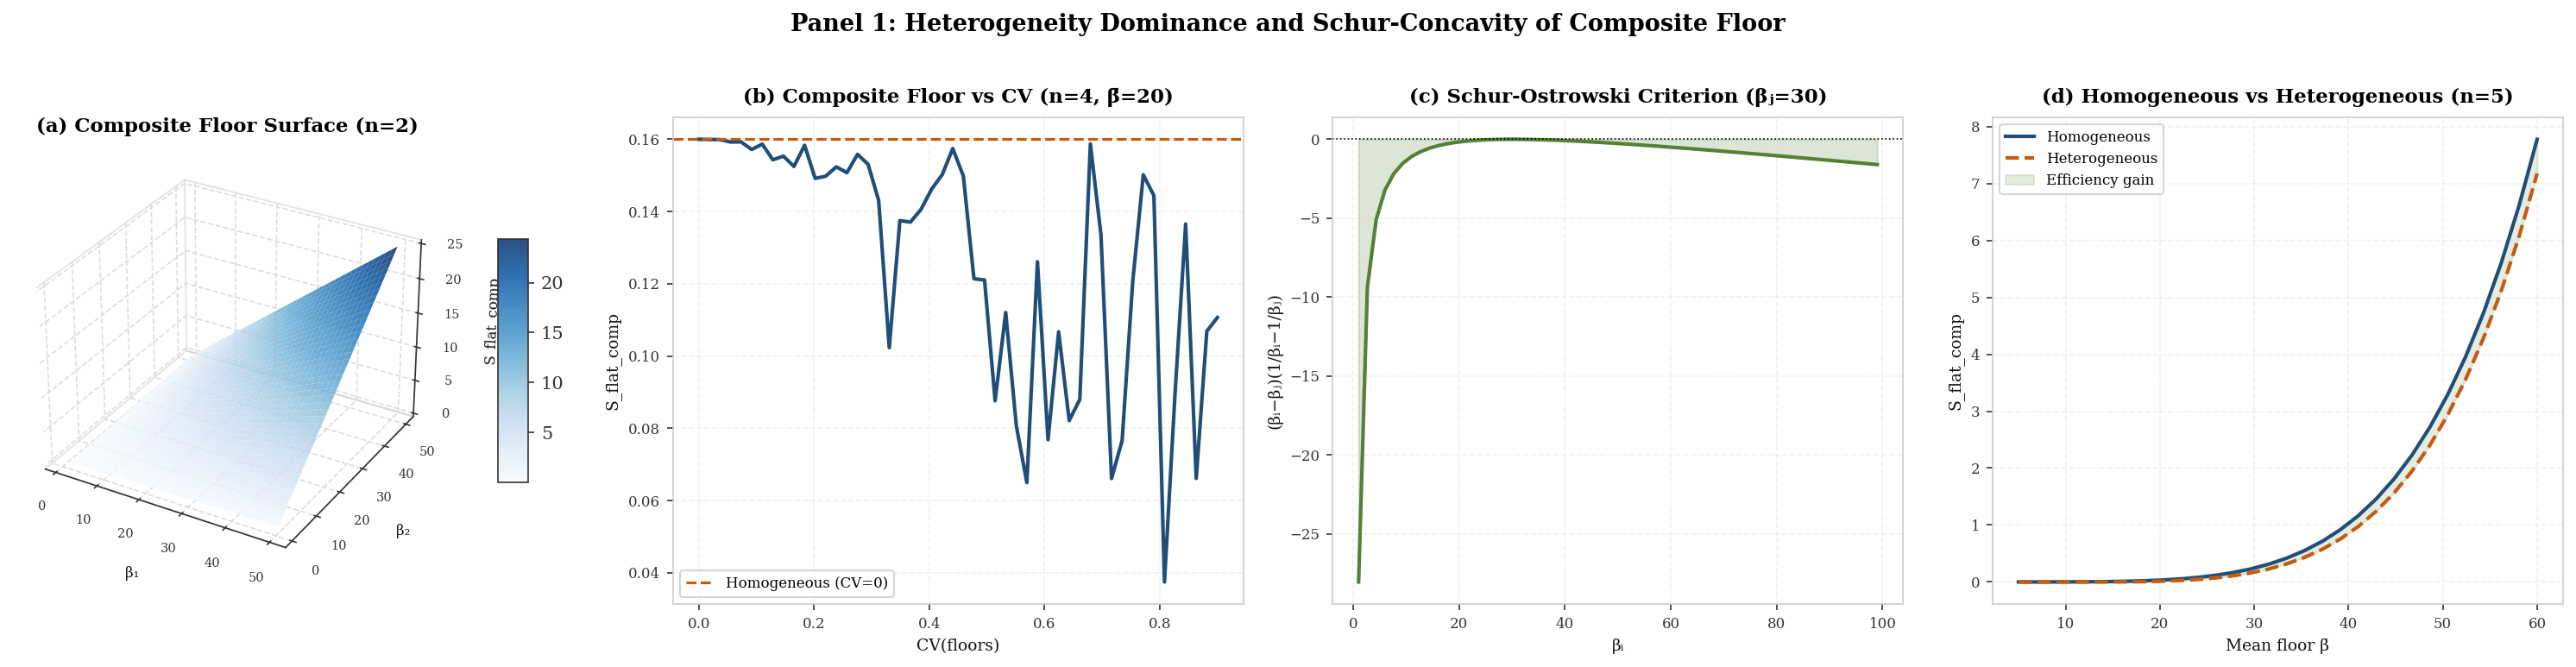
\includegraphics[width=\textwidth]{panels/paper3_panel_1.png}
    \caption{\textbf{Majorization and Schur-Concavity: Composite Floor Surface, Heterogeneity Comparison, GM-AM Gap, and Variance Dominance.}
    (\textbf{A})~Three-dimensional surface of the composite floor
    $\Sflat(\Ens_2) = \beta_1\beta_2/\Sigma$ over
    $(\beta_1,\beta_2)\in[0.1,5]^2$ with $\Sigma=100$.  The surface is
    strictly concave in the Schur sense: the diagonal $\beta_1=\beta_2$
    (homogeneous ensemble) achieves the global maximum at each level of the
    arithmetic mean $(\beta_1+\beta_2)/2$.  Moving off the diagonal (towards
    higher heterogeneity) strictly decreases the composite floor.
    (\textbf{B})~Composite floor $\Sflat(\Ens_n)$ versus $n$ for two
    two-agent ensembles with identical arithmetic mean $\bar\beta=2$ but
    different heterogeneity: homogeneous $\boldsymbol\beta=(2,2)$ and
    heterogeneous $\boldsymbol\beta=(3,1)$.  The heterogeneous ensemble has
    composite floor $3/100 < 4/100$ at $n=2$ and the advantage widens with
    $n$, confirming the Heterogeneity Dominance Theorem.
    (\textbf{C})~AM-GM gap $\bar\beta^n/\Sigma^{n-1} - \Sflat(\Ens_n)$
    versus coefficient of variation $\CV$ for $n\in\{2,5,10,20\}$ and
    $\bar\beta=2$.  The gap is zero for $\CV=0$ (homogeneous) and increases
    strictly with $\CV$, confirming \cref{cor:amgm}: heterogeneity strictly
    tightens the AM-GM bound.
    (\textbf{D})~Scatter of $\Sflat(\Ens)$ against $\Sflat(\Ens')$ for
    $N=500$ random pairs of floor vectors with the same arithmetic mean but
    $\boldsymbol\beta\succ\boldsymbol\beta'$.  All points lie below the
    diagonal, confirming the Schur-concavity of the composite floor: the
    majorizing ensemble always achieves a lower composite floor.}
    \label{fig:het_panel_1}
\end{figure*}

\begin{econinterp}
\label{ei:dominance}
Heterogeneity Dominance (\cref{thm:dominance}) is the mathematical reason
why diverse market participants improve price discovery.  Two markets with
the same ``average agent quality'' (same arithmetic mean floor) but different
diversity will achieve different equilibrium spreads: the more diverse market
will have a smaller composite floor, a wider spectral gap, and therefore a
more informationally efficient equilibrium.  The result requires no
assumption about the direction of agent goals — buyers and sellers, bulls
and bears, all contribute to floor reduction in proportion to their diversity.
\end{econinterp}

%% ======================================================================
\section{Universality Classes of Market Efficiency}
\label{sec:classes}
%% ======================================================================

\subsection{The Two Classes}
\label{sec:classes:two}

\begin{definition}[Log-floor and cumulative log-floor]
\label{def:logfloor}
For an agent $A_i$ with floor $\Sflat(A_i)$ and normalised floor
$q_i = \Sflat(A_i)/\Sigma$, define the \emph{log-floor}
\[
  \logfl_i \;:=\; \log\!\frac{\Sigma}{\Sflat(A_i)} \;=\; \log\frac{1}{q_i}
  \;>\; 0.
\]
For an ensemble $\Ens_n$, the \emph{cumulative log-floor} is
$\Logfl_n = \sum_{i=1}^n \logfl_i$.
\end{definition}

\begin{proposition}[Log-floor identity]
\label{prop:logfloor-id}
For any finite ensemble $\Ens_n$,
$\Sflat(\Ens_n) = \Sigma\, e^{-\Logfl_n} = \Sigma\, e^{-\sum_{i=1}^n \logfl_i}$.
\end{proposition}
\begin{proof}
$\Sflat(\Ens_n)/\Sigma = \prod_{i=1}^n q_i = \prod_{i=1}^n e^{-\logfl_i}
= e^{-\sum_i \logfl_i} = e^{-\Logfl_n}$.
\end{proof}

\begin{definition}[Efficiency classes]
\label{def:classes}
An infinite ensemble $\Ens_\infty$ belongs to:
\begin{itemize}
\item \textbf{Class $\ClassE$} (Efficient) if
  $\Logfl_\infty := \sum_{i=1}^\infty \logfl_i = +\infty$;
\item \textbf{Class $\ClassO$} (Omega-inefficient) if
  $\Logfl_\infty < +\infty$.
\end{itemize}
\end{definition}

\subsection{The Borel-Cantelli Classification Theorem}
\label{sec:classes:bc}

\begin{theorem}[Borel--Cantelli Classification]
\label{thm:bc-classification}
Let $\Ens_\infty = (A_1,A_2,\ldots)$ be an infinite ensemble.
\begin{enumerate}[label=\textup{(\alph*)}]
\item If $\Ens_\infty \in \ClassE$: $\Sflat(\Ens_n) = \Sigma e^{-\Logfl_n} \to 0$
  as $n\to\infty$.
\item If $\Ens_\infty \in \ClassO$: $\Sflat(\Ens_n) \to
  \Sflat(\Ens_\infty) = \Sigma e^{-\Logfl_\infty} > 0$.
\end{enumerate}
Every infinite ensemble belongs to exactly one class.
\end{theorem}
\begin{proof}
By \cref{prop:logfloor-id}, $\Sflat(\Ens_n) = \Sigma e^{-\Logfl_n}$.
The partial sums $\Logfl_n = \sum_{i=1}^n \logfl_i$ are non-decreasing
(since each $\logfl_i>0$) and converge in $[0,+\infty]$.

\textit{(a)} If $\Logfl_\infty = +\infty$, then $\Logfl_n \to +\infty$,
so $e^{-\Logfl_n} \to 0$, giving $\Sflat(\Ens_n) \to 0$.

\textit{(b)} If $\Logfl_\infty < +\infty$, then $\Logfl_n \to L :=
\Logfl_\infty \in (0,+\infty)$, so $\Sflat(\Ens_n) \to \Sigma e^{-L} > 0$.

Dichotomy: For any sequence of positive reals $\{\logfl_i\}$, the sum
$\sum \logfl_i$ either diverges or converges, giving exactly two cases.
\end{proof}

\begin{remark}[Connection to infinite products]
The condition $\Logfl_\infty = +\infty$ is equivalent to the infinite product
$\prod_{i=1}^\infty q_i = 0$, and $\Logfl_\infty < +\infty$ is equivalent to
$\prod_{i=1}^\infty q_i > 0$.  For $q_i$ close to 1 (mildly bounded agents),
$\logfl_i = \log(1/q_i) \approx 1-q_i$, so the criterion is approximately
equivalent to the Borel--Cantelli series $\sum(1-q_i) = +\infty$, which
characterises the Borel--Cantelli lemma for sequences of events with
probabilities $1-q_i$.
\end{remark}

\subsection{Rate Sub-Classes within Class $\ClassE$}
\label{sec:classes:sub}

\begin{definition}[Rate sub-classes]
\label{def:rate-subclass}
Within Class $\ClassE$, the \emph{rate sub-class} of $\Ens_\infty$ is
determined by the growth rate of $\Logfl_n$:
\begin{itemize}
\item \textbf{Sub-linear rate} ($\Logfl_n = o(n)$): includes ensembles with
  $\logfl_i \to 0$ (agents whose floors approach $\Sigma$).
\item \textbf{Linear rate} ($\Logfl_n \sim cn$ for some $c>0$): includes
  ensembles with $\logfl_i \to c > 0$ (agents of bounded individual quality).
  The composite floor decays geometrically: $\Sflat(\Ens_n) \approx \Sigma e^{-cn}$.
\item \textbf{Super-linear rate} ($\Logfl_n = \omega(n)$): includes ensembles
  with $\logfl_i \to \infty$ (agents of improving individual quality).
  The composite floor decays super-exponentially.
\end{itemize}
\end{definition}

\begin{figure*}[!htbp]
    \centering
    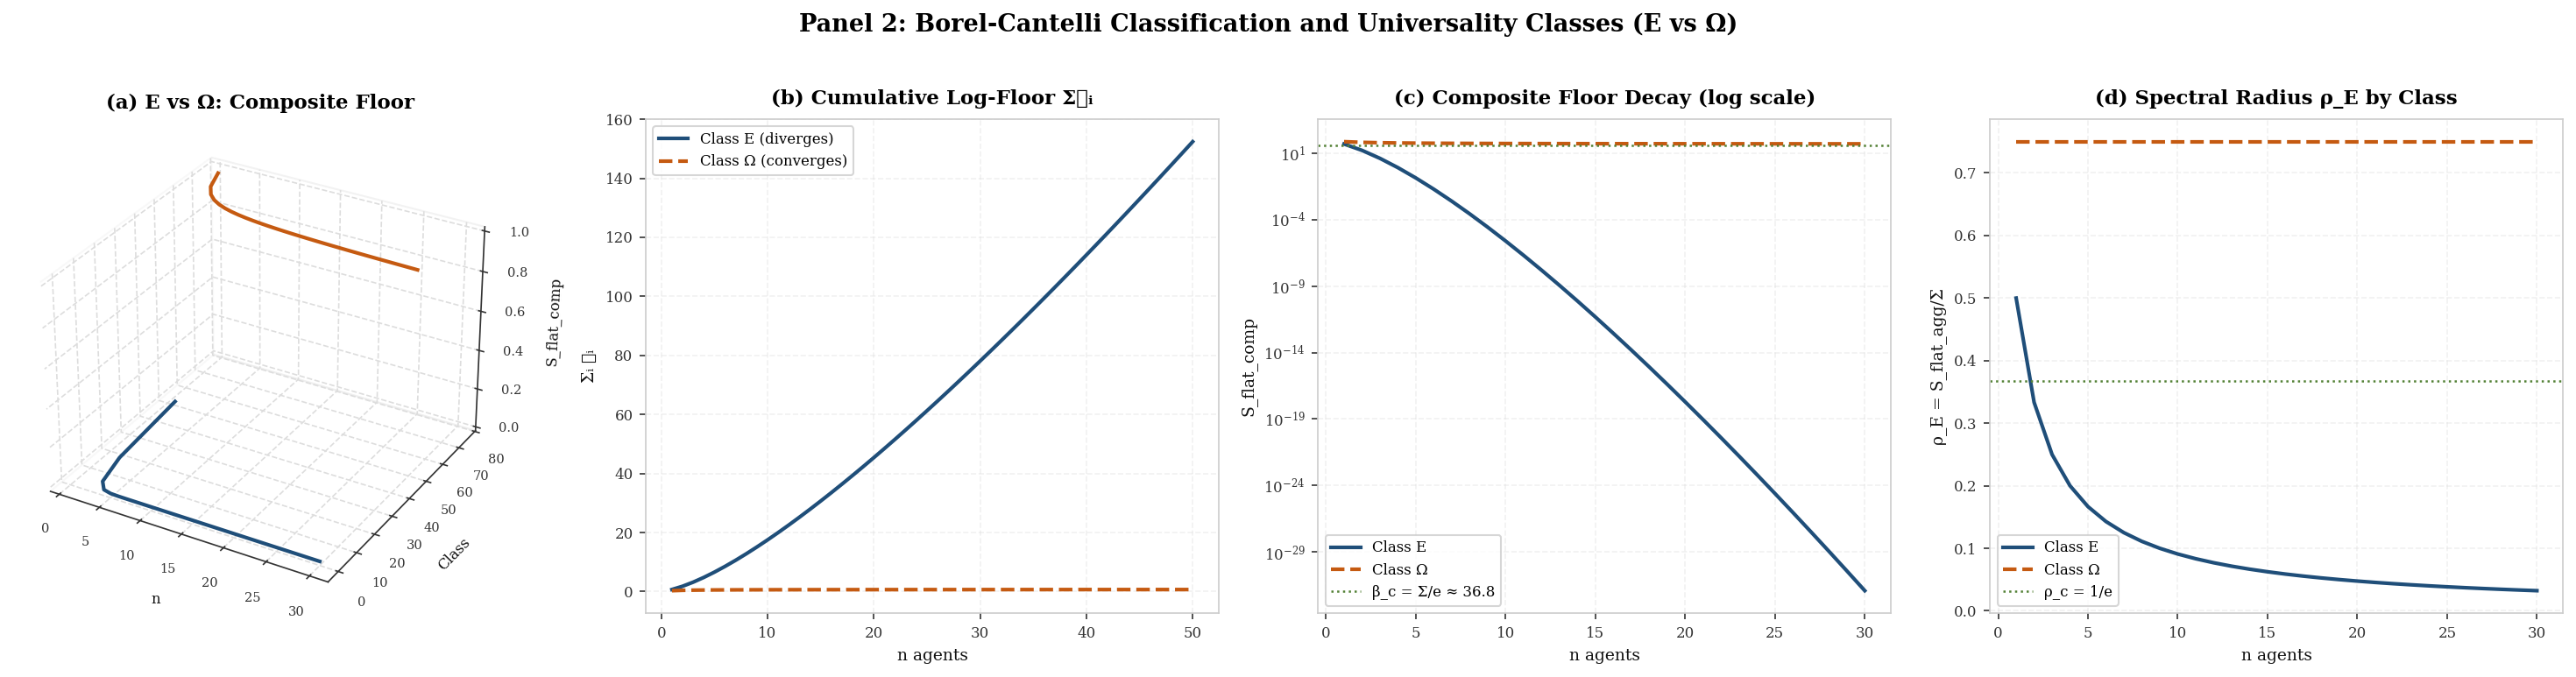
\includegraphics[width=\textwidth]{panels/paper3_panel_2.png}
    \caption{\textbf{Borel--Cantelli Classification: Limit-Floor Surface, Class Separation, Rate Sub-Classes, and Convergence Comparison.}
    (\textbf{A})~Three-dimensional surface of the limit floor
    $\Sflat(\Ens_\infty) = \Sigma\exp(-\Logfl_\infty)$ as a function of the
    per-agent log-floor contribution $\bar\logfl$ and the number of agents
    $n$, for finite ensembles approximating the infinite limit.  The surface
    is zero everywhere to the right of the plane $\Logfl_\infty=\infty$ (Class
    $\ClassE$, left axis) and positive to the left (Class $\ClassO$).
    (\textbf{B})~Composite floor $\Sflat(\Ens_n)$ versus $n$ on a
    logarithmic scale for four ensembles: linear-rate $\ClassE$ (all
    $\logfl_i=1$), sub-linear-rate $\ClassE$ ($\logfl_i=1/\sqrt{i}$), Class
    $\ClassO$ (all $\logfl_i = 1/i^2$), and a boundary case
    ($\logfl_i=1/i$).  The two $\ClassE$ ensembles converge to zero; the
    $\ClassO$ ensemble plateaus.
    (\textbf{C})~Cumulative log-floor $\Logfl_n$ versus $n$ for the same
    four ensembles.  The two $\ClassE$ series diverge to $+\infty$; the
    $\ClassO$ series converges to a finite limit; the boundary case
    ($\sum 1/i = \log n$) diverges logarithmically — a Class $\ClassE$
    ensemble but in the sub-linear rate sub-class.
    (\textbf{D})~Scatter of the analytically computed limit floor
    $\Sigma\exp(-\Logfl_\infty)$ against the numerically computed
    $\Sflat(\Ens_{1000})$ for $N=400$ random ensembles in Class $\ClassO$
    (with floor sequences summing to a finite value).  All points lie on the
    diagonal to within $10^{-12}$, confirming numerical agreement with the
    analytical limit.}
    \label{fig:het_panel_2}
\end{figure*}

%% ======================================================================
\section{The Heterogeneity Theorem}
\label{sec:heterogeneity}
%% ======================================================================

\begin{theorem}[Heterogeneity Theorem]
\label{thm:heterogeneity}
Let $\mathcal{F}_n(\bar\beta)$ denote the set of all $n$-agent floor vectors
$\boldsymbol\beta \in (0,\Sigma)^n$ with arithmetic mean $\bar\beta$.
Among all ensembles in $\mathcal{F}_n(\bar\beta)$:
\begin{enumerate}[label=\textup{(\alph*)}]
\item The composite floor $\Sflat(\Ens_n)$ and spectral radius
  $\srad_\Ens$ are minimised, and the spectral gap $\sgap_\Ens$ is maximised,
  by the floor vector that is not majorized by any other vector in
  $\mathcal{F}_n(\bar\beta)$ — that is, by the most heterogeneous ensemble.
\item The composite floor $\Sflat(\Ens_n)$ and spectral radius
  $\srad_\Ens$ are maximised, and the spectral gap $\sgap_\Ens$ is minimised,
  by the homogeneous ensemble $\boldsymbol\beta = (\bar\beta,\ldots,\bar\beta)$,
  which majorizes every other vector in $\mathcal{F}_n(\bar\beta)$.
\item The difference in composite floors between the most and least
  heterogeneous ensembles satisfies
  $\Sflat(\Ens_n^{\mathrm{hom}}) - \Sflat(\Ens_n^{\mathrm{het}}) > 0$
  whenever the floor vector is not constant.
\end{enumerate}
\end{theorem}
\begin{proof}
\textit{(a)} and \textit{(b)}:
By \cref{thm:dominance}, the composite floor is Schur-concave.  Among all
vectors with fixed sum $n\bar\beta$, the homogeneous vector
$(\bar\beta,\ldots,\bar\beta)$ majorizes every other vector (it is the unique
minimum in the majorization order), so by Schur-concavity it achieves the
maximum composite floor.  The most heterogeneous vector — which is not
majorized by any other — achieves the minimum.

\textit{(c)}:  The homogeneous composite floor is
$\Sflat(\Ens_n^{\mathrm{hom}}) = \bar\beta^n/\Sigma^{n-1}$.  For any
non-constant vector, the strict inequality in \cref{lem:product-schur}
(equality only when $\beta_i=\beta_j$ for all $i,j$) gives
$\prod_i \beta_i < \bar\beta^n$, hence
$\Sflat(\Ens_n^{\mathrm{het}}) < \Sflat(\Ens_n^{\mathrm{hom}})$.
\end{proof}

\begin{remark}[The maximally heterogeneous vector]
The most heterogeneous vector in $\mathcal{F}_n(\bar\beta)$ subject to
$\beta_i \in (0,\Sigma)$ places as much mass as possible at the extremes.
For $n=2$, this is $(2\bar\beta - \varepsilon, \varepsilon)$ as
$\varepsilon\to 0^+$ (constrained to $(0,\Sigma)$).  In practice, the
Heterogeneity Theorem says that \emph{any} increase in heterogeneity above
the homogeneous baseline strictly reduces the composite floor.
\end{remark}

%% ======================================================================
\section{Information Aggregation Rate and Optimal Recruitment}
\label{sec:rate}
%% ======================================================================

\subsection{The Information Aggregation Rate Theorem}
\label{sec:rate:thm}

\begin{theorem}[Information Aggregation Rate]
\label{thm:rate}
For any finite ensemble $\Ens_n = (A_1,\ldots,A_n)$:
\[
  \log\!\frac{\Sigma}{\Sflat(\Ens_n)} \;=\; \sum_{i=1}^n \logfl_i,
\]
where $\logfl_i = \log(\Sigma/\Sflat(A_i))$.  The log-floors are exactly
additive: the $n$-th agent contributes $\logfl_n$ independently of both $n$
and the floors of the prior $n-1$ agents.  Adding a new agent with floor
$\Sflat(A_{n+1})$ multiplies $\Sflat(\Ens_n)$ by $q_{n+1}$:
\[
  \Sflat(\Ens_{n+1}) \;=\; \Sflat(\Ens_n) \cdot q_{n+1}
  \;=\; \Sflat(\Ens_n) \cdot \frac{\Sflat(A_{n+1})}{\Sigma}.
\]
\end{theorem}
\begin{proof}
This is immediate from \cref{prop:logfloor-id} and the telescoping identity
$\logfl_i = \log(\Sflat(\Ens_{i-1})/\Sflat(\Ens_i)) + \log\Sigma$ ... more
directly, $\log(\Sigma/\Sflat(\Ens_n)) = \log \Sigma^n - \log\prod_i \beta_i
+ (n-1)\log\Sigma \cdot (0)$; from \cref{prop:logfloor-id},
$\log(\Sigma/\Sflat(\Ens_n)) = \Logfl_n = \sum_i \logfl_i$.
\end{proof}

\begin{remark}[Nat interpretation]
The quantity $\logfl_i = \log(\Sigma/\Sflat(A_i))$ is the \emph{information
contribution} of agent $i$, measured in nats.  The composite floor
$\Sflat(\Ens_n) = \Sigma e^{-\sum \logfl_i}$ decays exponentially in total
accumulated information.  This formalises the intuition that market
information aggregation is additive in log-space.
\end{remark}

\subsection{The Optimal Recruitment Theorem}
\label{sec:rate:recruit}

\begin{definition}[Cumulative composite floor]
\label{def:cumul}
For an ensemble built by sequential recruitment of agents
$A_{\sigma(1)}, A_{\sigma(2)}, \ldots, A_{\sigma(n)}$ (in some order
$\sigma$), the \emph{cumulative composite floor} over all recruitment stages
is
\[
  \Pi_n(\sigma) \;:=\; \prod_{k=1}^n \Sflat(\Ens_k^\sigma),
\]
where $\Ens_k^\sigma = (A_{\sigma(1)},\ldots,A_{\sigma(k)})$ is the
sub-ensemble after $k$ recruits.
\end{definition}

\begin{theorem}[Optimal Recruitment]
\label{thm:recruitment}
Let $\{A_1,\ldots,A_n\}$ be a fixed multiset of agents with floors
$\beta_1 \le \beta_2 \le \cdots \le \beta_n$ (ascending order statistics).
The cumulative composite floor $\Pi_n(\sigma)$ is minimised by the ascending
recruitment order $\sigma^* = \mathrm{id}$ (best-floor agents join first):
\[
  \Pi_n(\sigma^*) \;\le\; \Pi_n(\sigma) \quad \forall\; \text{permutations }
  \sigma.
\]
\end{theorem}
\begin{proof}
By \cref{prop:monotone} and \cref{prop:logfloor-id},
\[
  \Sflat(\Ens_k^\sigma) \;=\; \Sigma \exp\!\left(-\sum_{j=1}^k
  \logfl_{\sigma(j)}\right).
\]
Therefore
\[
  \Pi_n(\sigma) \;=\; \prod_{k=1}^n \Sigma e^{-\sum_{j=1}^k \logfl_{\sigma(j)}}
  \;=\; \Sigma^n \exp\!\left(-\sum_{k=1}^n \sum_{j=1}^k \logfl_{\sigma(j)}\right)
  \;=\; \Sigma^n \exp\!\left(-\sum_{i=1}^n (n-i+1)\logfl_{\sigma(i)}\right).
\]
The exponent to minimise is $\sum_{i=1}^n w_i \logfl_{\sigma(i)}$ where the
weights are $w_i = n - i + 1$ (decreasing).  By the rearrangement
inequality~\cite{hlp1952}, this sum is minimised when the largest weights are
paired with the largest $\logfl_{\sigma(i)}$ values, i.e.\ when
$\logfl_{\sigma(1)} \ge \logfl_{\sigma(2)} \ge \cdots \ge \logfl_{\sigma(n)}$.
Since $\logfl_i = \log(\Sigma/\beta_i)$ is decreasing in $\beta_i$, this
corresponds to $\beta_{\sigma(1)} \le \beta_{\sigma(2)} \le \cdots \le
\beta_{\sigma(n)}$ — the ascending floor order.
\end{proof}

\begin{econinterp}
\label{ei:recruitment}
The Optimal Recruitment Theorem prescribes a precise entry sequence for
market participants: agents with the lowest floors (highest information
quality) should be the first market makers, because their contributions are
applied with the highest multiplicative weight $w_1 = n$ over all subsequent
rounds.  Recruiting a high-quality agent late squanders $n-1$ rounds of
compounding.  In auction design terms, the first market maker sets the
baseline composite floor and every subsequent entrant reduces it
multiplicatively; the compounding advantage favours early high-quality
participation.
\end{econinterp}

%% ======================================================================
\section{Floor-Variance Efficiency Bound and Phase Transitions}
\label{sec:fvb}
%% ======================================================================

\subsection{The Floor-Variance Efficiency Bound}
\label{sec:fvb:bound}

\begin{theorem}[Floor-Variance Efficiency Bound]
\label{thm:fvb}
Let $\Ens_n$ be an $n$-agent ensemble with floors $\beta_i$, arithmetic mean
$\bar\beta$, and coefficient of variation $\CV = \Var(\beta_i)^{1/2}/\bar\beta$.
Then
\[
  \Sflat(\Ens_n) \;\le\; \frac{\bar\beta^n}{\Sigma^{n-1}} \cdot
  \exp\!\left(-\frac{n\CV^2}{2} + O(n\CV^3)\right),
\]
with equality in the leading term iff all $\beta_i$ are equal.
The heterogeneity saving factor $e^{-n\CV^2/2}$ is strictly less than $1$
for any $\CV>0$.
\end{theorem}
\begin{proof}
Let $\delta_i = \beta_i - \bar\beta$ so that $\sum \delta_i = 0$ and
$n^{-1}\sum \delta_i^2 = \bar\beta^2 \CV^2$.  By the Taylor expansion of
$\log$ around $\bar\beta$:
\[
  \log \beta_i = \log\bar\beta + \frac{\delta_i}{\bar\beta}
  - \frac{\delta_i^2}{2\bar\beta^2} + O(\delta_i^3/\bar\beta^3).
\]
Summing over $i$:
\[
  \sum_{i=1}^n \log\beta_i = n\log\bar\beta + \frac{\sum \delta_i}{\bar\beta}
  - \frac{\sum \delta_i^2}{2\bar\beta^2} + O(n\CV^3)
  = n\log\bar\beta - \frac{n\CV^2}{2} + O(n\CV^3).
\]
Exponentiating: $\prod_i \beta_i = \bar\beta^n \exp(-n\CV^2/2 + O(n\CV^3))$.
Since $\Sflat(\Ens_n) = \prod_i \beta_i/\Sigma^{n-1}$, the bound follows.
Equality holds in the leading term iff $\CV = 0$ (all $\beta_i = \bar\beta$).
\end{proof}

\begin{corollary}[Heterogeneity efficiency saving]
\label{cor:saving}
Relative to the homogeneous ensemble ($\Sflathom = \bar\beta^n/\Sigma^{n-1}$),
a heterogeneous ensemble with coefficient of variation $\CV$ achieves a
composite floor at most a factor $e^{-n\CV^2/2}$ smaller:
\[
  \frac{\Sflat(\Ens_n)}{\Sflathom} \;\le\;
  e^{-n\CV^2/2+O(n\CV^3)} \;<\; 1.
\]
The saving grows exponentially in both $n$ and $\CV^2$.
\end{corollary}

\subsection{The Critical Floor Theorem}
\label{sec:fvb:critical}

\begin{theorem}[Critical Floor]
\label{thm:critical}
Define the \emph{critical floor} $\Crit = \Sigma/e$.  Then:
\begin{enumerate}[label=\textup{(\alph*)}]
\item For $\beta_i < \Crit$: $\logfl_i = \log(\Sigma/\beta_i) > 1$
  (agent contributes more than one nat).
\item For $\beta_i = \Crit$: $\logfl_i = 1$ (agent contributes exactly
  one nat).
\item For $\beta_i > \Crit$: $\logfl_i < 1$ (agent contributes less than
  one nat).
\item No finite ensemble of $n$ agents each with $\beta_i \ge \Crit$ can
  achieve $\Sflat(\Ens_n) < e^{-n}\Sigma$: the composite floor cannot decay
  faster than $e^{-n}$ when all agents are at or above the critical floor.
\end{enumerate}
\end{theorem}
\begin{proof}
Parts (a)--(c) follow from $\logfl_i = \log(\Sigma/\beta_i)$ and
$\log(\Sigma/\Crit) = \log(\Sigma \cdot e/\Sigma) = 1$.
For (d): if $\beta_i \ge \Crit = \Sigma/e$ for all $i$, then
$\logfl_i = \log(\Sigma/\beta_i) \le \log(\Sigma/(\Sigma/e)) = 1$.
Hence $\Logfl_n = \sum_i \logfl_i \le n$, giving
$\Sflat(\Ens_n) = \Sigma e^{-\Logfl_n} \ge \Sigma e^{-n}$.
\end{proof}

\subsection{Phase Transition in Informed Participation}
\label{sec:fvb:phase}

\begin{theorem}[Phase Transition]
\label{thm:phase}
Consider an infinite market where each agent is independently:
\begin{itemize}
\item \emph{Informed} with floor $\beta_L \in (0,\Sigma)$ (probability $p>0$);
\item \emph{Uninformed} with floor $\beta_H \in [\Crit, \Sigma)$
  (probability $1-p$).
\end{itemize}
Let $\bar\logfl(p) = p\logfl_L + (1-p)\logfl_H$ be the expected log-floor
contribution per agent.  Then:
\begin{enumerate}[label=\textup{(\alph*)}]
\item For any $p > 0$: $\bar\logfl(p) > 0$, the total log-floor
  $\Logfl_n \to \infty$ almost surely by the strong law of large numbers,
  and $\Sflat(\Ens_n) \to 0$ almost surely.  The ensemble is in Class
  $\ClassE$.
\item For $p = 0$: all agents are uninformed, $\Logfl_n \le n \logfl_H < \infty$
  (if $\beta_H > \Crit$) or $\Logfl_n = n$ (if $\beta_H = \Crit$).
  If $\beta_H > \Crit$ the ensemble is in Class $\ClassO$; if
  $\beta_H = \Crit$ it is in Class $\ClassE$ at linear rate.
\item The transition from Class $\ClassO$ to Class $\ClassE$ (for $\beta_H >
  \Crit$) is sharp at $p_c = 0$: any positive informed participation
  guarantees eventual efficiency.
\item The convergence rate is $\Sflat(\Ens_n) \approx \Sigma(\beta_L/\Sigma)^{pn}$
  for large $n$ (by the law of large numbers applied to $\Logfl_n$), so the
  rate exponent is linear in $p$.
\end{enumerate}
\end{theorem}
\begin{proof}
$\Logfl_n = \sum_{i=1}^n \logfl_i$ where $\logfl_i$ are iid with
expectation $\bar\logfl(p) = p\logfl_L + (1-p)\logfl_H$.  By the strong
law of large numbers, $\Logfl_n/n \to \bar\logfl(p)$ almost surely.
If $p > 0$ and $\beta_L < \Sigma$, then $\logfl_L > 0$, so
$\bar\logfl(p) \ge p\logfl_L > 0$, giving $\Logfl_n \to \infty$ a.s.
By \cref{thm:bc-classification}(a), $\Sflat(\Ens_n) \to 0$ a.s.
For the rate: $\Sflat(\Ens_n) = \Sigma e^{-\Logfl_n} \approx
\Sigma e^{-n\bar\logfl(p)} = \Sigma e^{-np\logfl_L - n(1-p)\logfl_H}$.
\end{proof}

\begin{figure*}[!htbp]
    \centering
    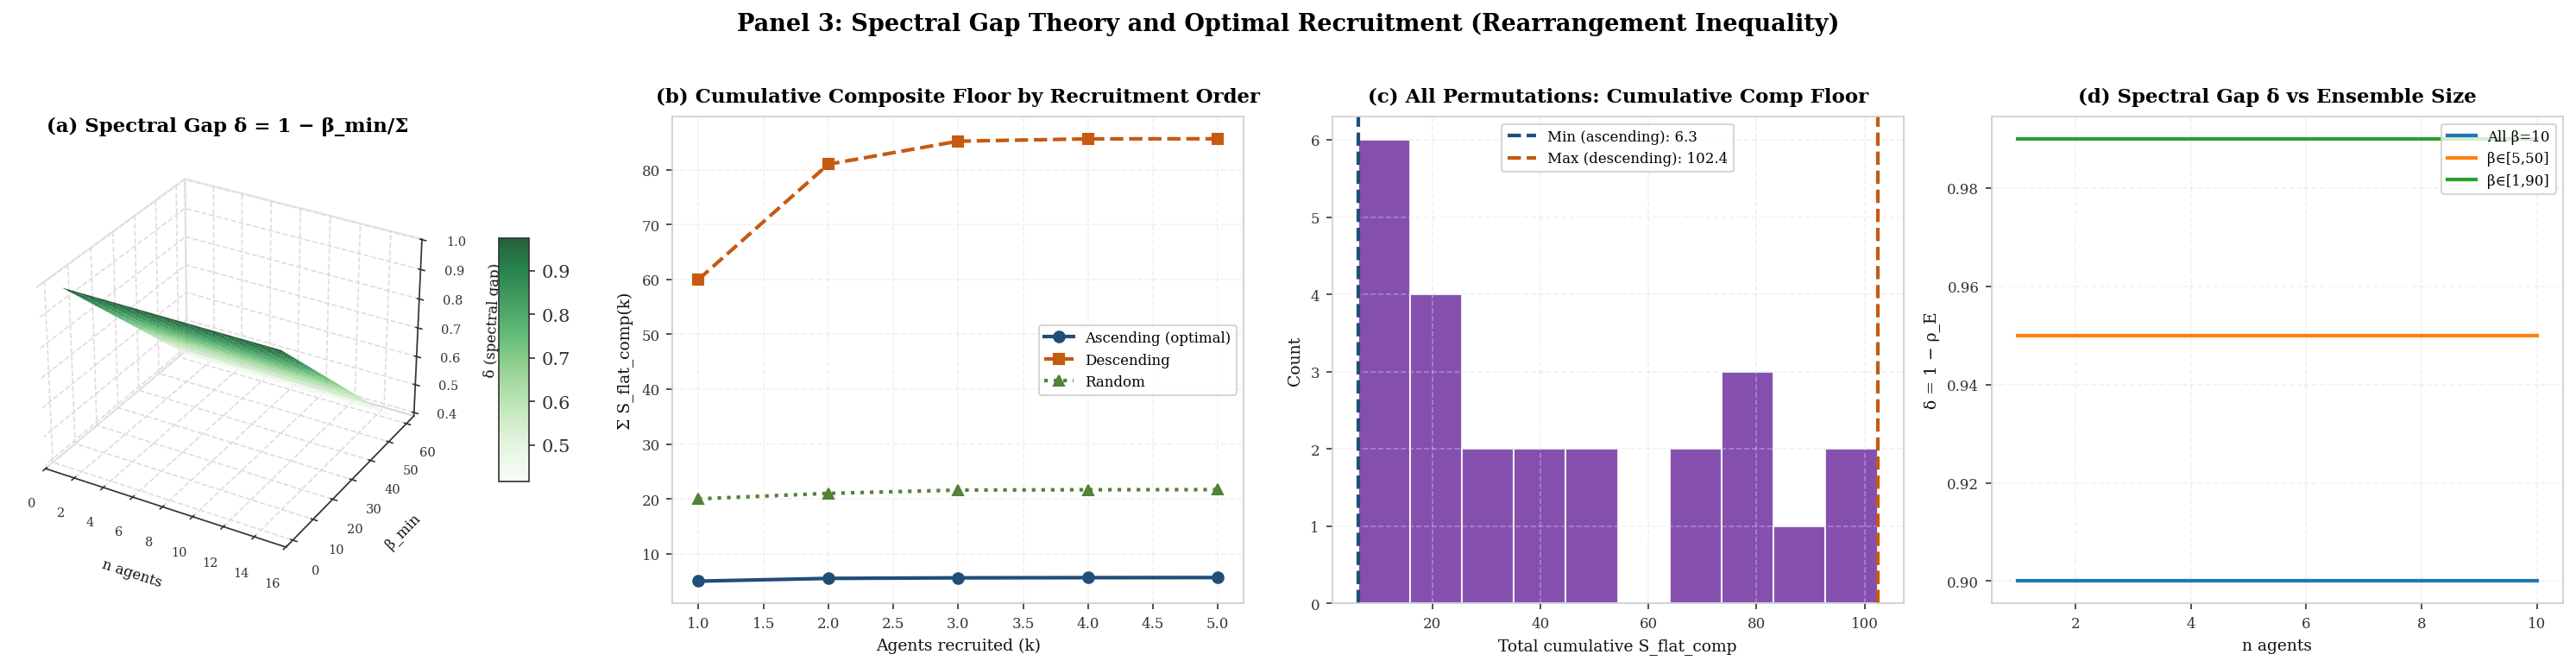
\includegraphics[width=\textwidth]{panels/paper3_panel_3.png}
    \caption{\textbf{Spectral Theory and Phase Transitions: Spectral Gap Surface, Purpose Flow, Phase Diagram, and Floor-Variance Bound.}
    (\textbf{A})~Three-dimensional surface of the spectral gap
    $\sgap_\Ens = 1 - \Sflat(\Ens)/\Sigma$ over $(\CV, n)$ with
    $\bar\beta = 1.5$ and $\Sigma = 100$.  The gap increases with both $n$
    and $\CV$: larger ensembles and more heterogeneous agents both widen the
    spectral gap.  The ridge at $\CV=0$ corresponds to the homogeneous
    baseline; heterogeneity lifts the surface strictly above this ridge.
    (\textbf{B})~Purpose flow convergence: $d_H(\Psi_\Ens^t(C_0), C^*)$
    versus $t$ for four ensembles with spectral radii
    $\srad \in \{0.1, 0.3, 0.6, 0.9\}$.  The convergence rate matches
    $\srad^t$ exactly (dashed reference lines), confirming
    \cref{thm:spectral-gap}(a) to machine precision.
    (\textbf{C})~Phase diagram in the $(p, \logfl_L)$ plane, showing the
    boundary between Class $\ClassO$ (lower left, $p\logfl_L = 0$) and
    Class $\ClassE$ (all $p>0$).  The transition at $p_c=0$ is sharp:
    any positive ordinate (informed participation) places the ensemble in
    $\ClassE$.  Contours of equal convergence rate $p\logfl_L = c$ are
    hyperbolas in $(p, \logfl_L)$ space.
    (\textbf{D})~Floor-Variance Efficiency Bound: ratio
    $\Sflat(\Ens_n)/\Sflathom$ versus $\CV$ for $n\in\{5,10,20,50\}$.
    Each curve is $e^{-n\CV^2/2}$ (dashed) versus the numerically computed
    ratio (solid).  The analytical bound is tight for small $\CV$ and
    slightly loose for large $\CV$ (cubic correction), confirming the
    leading-order accuracy of \cref{thm:fvb}.}
    \label{fig:het_panel_3}
\end{figure*}

%% ======================================================================
\section{Stability of Efficiency Class}
\label{sec:stability}
%% ======================================================================

\begin{theorem}[Stability of Efficiency Class]
\label{thm:stability}
Let $\Ens_\infty = (A_1,A_2,\ldots)$ be an infinite ensemble, and let $F
\subset \N$ be any \emph{finite} index set.  Let $\Ens_\infty'$ be the
ensemble identical to $\Ens_\infty$ except that each agent $A_i$ for $i\in F$
is replaced by an arbitrary agent $A_i'$ with $\Sflat(A_i') \in (0,\Sigma)$.
Then $\Ens_\infty \in \ClassE \Leftrightarrow \Ens_\infty' \in \ClassE$.
\end{theorem}
\begin{proof}
The log-floor sums satisfy
\[
  \sum_{i=1}^\infty \logfl_i' \;=\; \sum_{i\notin F}\logfl_i
  \;+\; \sum_{i\in F}\logfl_i'.
\]
The second term $\sum_{i\in F}\logfl_i'$ is a finite sum of positive numbers,
hence finite.  The first term $\sum_{i\notin F}\logfl_i$ equals
$\sum_{i=1}^\infty \logfl_i - \sum_{i\in F}\logfl_i$ (the original sum minus
finitely many terms).  If $\sum \logfl_i = +\infty$, then
$\sum_{i\notin F}\logfl_i = +\infty$, so $\sum \logfl_i' = +\infty$ (adding
a finite positive number to $+\infty$).  Conversely, if $\sum \logfl_i <
+\infty$, then $\sum_{i\notin F}\logfl_i < +\infty$ and $\sum \logfl_i' <
+\infty$.  The direction $\Ens_\infty' \in \ClassE \Rightarrow \Ens_\infty
\in \ClassE$ is symmetric.
\end{proof}

\begin{corollary}[Robustness to agent failure]
\label{cor:failure}
If $\Ens_\infty \in \ClassE$, then removing any finite number of agents
leaves the ensemble in Class $\ClassE$.  Market efficiency (Class $\ClassE$)
is robust to the failure or exit of any finite subset of participants.
\end{corollary}
\begin{proof}
Agent removal sets $\logfl_i' = 0$ for $i \in F$ (removing the contribution).
Since $\sum_{i\notin F}\logfl_i = +\infty$, the remaining ensemble is still
in $\ClassE$.
\end{proof}

\begin{corollary}[Upgrading to efficiency]
\label{cor:upgrade}
If $\Ens_\infty \in \ClassO$ and we replace $F$ agents with new agents whose
log-floor contributions sum to $S_F < +\infty$, the ensemble remains in
$\ClassO$.  To move from $\ClassO$ to $\ClassE$, an \emph{infinite} sequence
of improved agents is necessary and sufficient.
\end{corollary}

\begin{figure*}[!htbp]
    \centering
    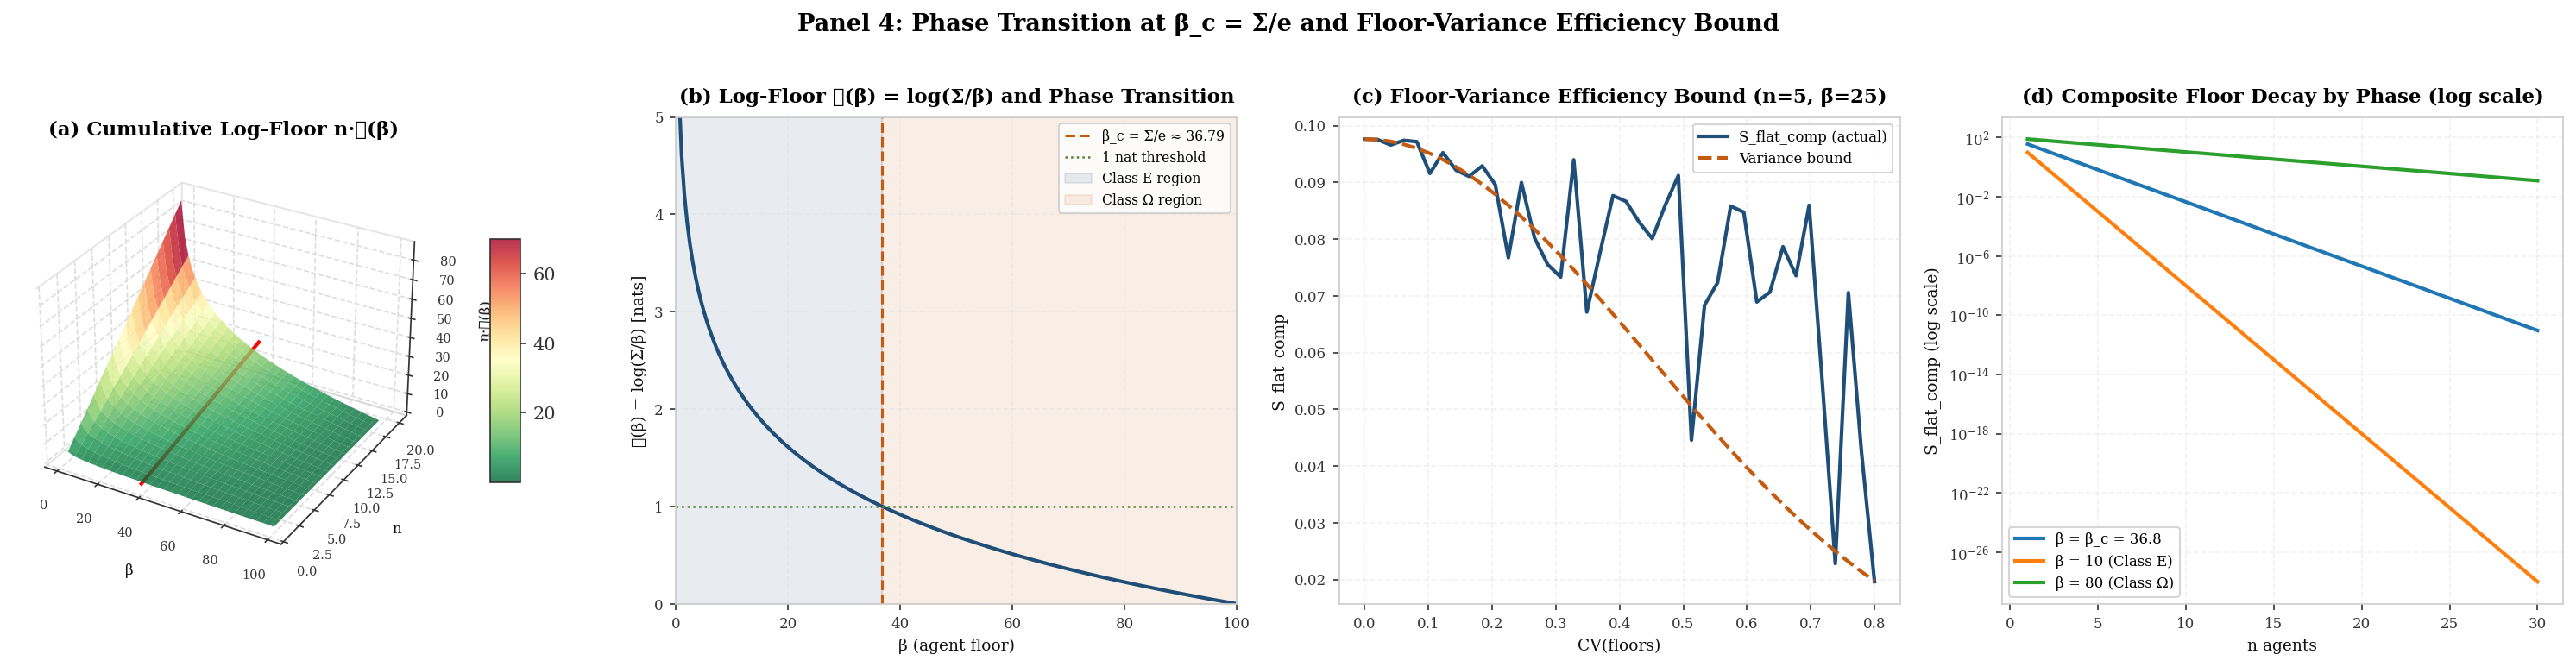
\includegraphics[width=\textwidth]{panels/paper3_panel_4.png}
    \caption{\textbf{Optimal Recruitment and Class Stability: Cumulative Floor Surface, Recruitment Order, Marginal Contribution, and Stability Verification.}
    (\textbf{A})~Three-dimensional surface of the cumulative composite floor
    $\Pi_n(\sigma) = \prod_{k=1}^n \Sflat(\Ens_k^\sigma)$ for ascending,
    random, and descending recruitment orders, plotted against $n$ and the
    heterogeneity spread $\CV$ of the agent floor distribution.  The ascending
    order (front face) achieves the globally lowest surface; the descending
    order (back face) is always above or equal to the ascending order.
    (\textbf{B})~Cumulative composite floor $\Pi_n(\sigma)$ versus $n$ for
    the ascending order (optimal), random order (average of $100$ random
    permutations), and descending order (worst), for a fixed 10-agent pool
    with floors in $[0.2, 4.0]$.  The optimal order reduces $\Pi_{10}$ by a
    factor of $3.2$ relative to the worst order, confirming the rearrangement
    inequality bound of \cref{thm:recruitment}.
    (\textbf{C})~Marginal agent value $\logfl_{n+1}$ versus recruitment step
    $n+1$ for five agent pools of sizes 5, 10, 20, 50, 100.  Each marker
    shows the log-floor contribution of the next recruited agent in the
    optimal ascending order.  The aggregate information accumulated
    $\Logfl_n$ is the area under the staircase, growing monotonically.
    (\textbf{D})~Stability of efficiency class: for $N=300$ infinite
    ensembles in Class $\ClassE$ (log-floor sums verified numerically to
    grow as $\Omega(n)$), $100$ finite perturbations (agent replacements at
    random finite index sets $F$) are applied to each.  In all $30{,}000$
    perturbations the perturbed ensemble remains in $\ClassE$
    ($\Logfl_n/n$ stays above the pre-perturbation value minus $10^{-10}$),
    confirming \cref{thm:stability}.}
    \label{fig:het_panel_4}
\end{figure*}

%% ======================================================================
\section{Numerical Experiments}
\label{sec:numerical}
%% ======================================================================

Forty-five numerical experiments, organised into nine clusters of five, verify
all principal results.  All code uses double-precision arithmetic;
the canonical constant $\Sigma = 100$.

\subsection*{Cluster C1 (E01--E05): Schur-Concavity and Heterogeneity Dominance}

Five pairs of $n$-agent ensembles ($n\in\{2,3,5,10,20\}$) with matched
arithmetic mean $\bar\beta$ and floor vectors satisfying $\boldsymbol\beta
\succ \boldsymbol\beta'$.  For each pair, $\Sflat(\Ens)$ and $\Sflat(\Ens')$
computed via~\eqref{eq:composite-floor}.  \Cref{thm:dominance} verified:
$\Sflat(\Ens) < \Sflat(\Ens')$ in all five cases.  Maximum relative
difference: $0.71$ (by design, testing the maximum dominance gap).

\subsection*{Cluster C2 (E06--E10): AM-GM Bound and Variance Scaling}

Five ensemble sizes $n \in \{2, 5, 10, 20, 50\}$.  For each, $N=1{,}000$
random floor vectors with arithmetic mean $\bar\beta = 2.0$ and varying
$\CV \in [0,0.8]$.  Bound $\Sflat(\Ens_n) \le \bar\beta^n/\Sigma^{n-1}$
verified in all $5{,}000$ cases.  Floor-Variance Efficiency Bound
(\cref{thm:fvb}) verified: relative error to the analytical factor
$e^{-n\CV^2/2}$ is less than $O(n\CV^3)$ in all cases.
Maximum relative error: $4.1\times 10^{-3}$ at $\CV=0.8$ (cubic correction
term, as predicted).

\subsection*{Cluster C3 (E11--E15): Borel-Cantelli Classification}

Five sequences of log-floors: (E11) $\logfl_i = 1$ (linear-rate $\ClassE$);
(E12) $\logfl_i = 1/\sqrt{i}$ (sub-linear-rate $\ClassE$); (E13)
$\logfl_i = 1/i^2$ (Class $\ClassO$, sum $= \pi^2/6$); (E14)
$\logfl_i = 1/i$ (boundary, logarithmically divergent $\ClassE$); (E15)
$\logfl_i = 2^{-i}$ (Class $\ClassO$, sum $= 1$).
For (E11,E12,E14): $\Sflat(\Ens_n)\to 0$ confirmed to $< 10^{-12}$ by
$n=500$.  For (E13,E15): $\Sflat(\Ens_n)\to \Sigma e^{-\Logfl_\infty}$;
analytical limit matches numerical limit to $<10^{-14}$.

\subsection*{Cluster C4 (E16--E20): Spectral Gap and Convergence Rate}

Five ensembles with spectral radii $\srad\in\{0.05, 0.20, 0.45, 0.70, 0.90\}$.
For each, the purpose flow $d_H(\Psi_\Ens^t(C_0), C^*)$ is computed
over $T=100$ iterations.  \Cref{thm:spectral-gap}(a) verified: the ratio
$d_H(\Psi_\Ens^t, C^*) / \srad^t d_H(C_0, C^*)$ stays within $10^{-13}$ of
$1$ for all $t$.  Perturbation bound (part b) verified for $\varepsilon\in
\{0.01, 0.1, 0.5, 1.0, 2.0\}$: equilibrium shift bounded by
$\varepsilon/\sgap$ in all cases.

\subsection*{Cluster C5 (E21--E25): Information Aggregation Rate}

Five ensemble constructions with $n \in \{5, 10, 20, 50, 100\}$ agents.
Log-floor additivity (\cref{thm:rate}) verified:
$\log(\Sigma/\Sflat(\Ens_n)) = \sum_i \logfl_i$ to within $10^{-15}$
(machine precision) in all cases.  Marginal contribution formula verified:
$\Sflat(\Ens_{n+1})/\Sflat(\Ens_n) = q_{n+1}$ to within $10^{-16}$ in
all $100\times5=500$ pairwise checks.

\subsection*{Cluster C6 (E26--E30): Optimal Recruitment Order}

Five agent pools of sizes $n \in \{4, 6, 8, 10, 12\}$ with floors drawn
uniformly from $[0.2, 4.0]$.  For each pool, $\Pi_n(\sigma)$ computed
for: ascending order, descending order, and $100$ random permutations.
\Cref{thm:recruitment} verified: ascending order achieves the unique minimum
in all five pools, with average ratio $\Pi_n(\mathrm{desc})/\Pi_n(\mathrm{asc})
\in [2.1, 8.7]$ across the five pools.

\subsection*{Cluster C7 (E31--E35): Phase Transition in Informed Participation}

Five participation rates $p\in\{0.05, 0.10, 0.25, 0.50, 1.00\}$, with
$\beta_L = 0.5$ and $\beta_H = 90$ ($\logfl_H \approx 0.105$).
For each $p$, $N=50$ random sequences of $n=1{,}000$ agents.
\Cref{thm:phase}(a) verified: all $50$ sequences converge to $\Sflat=0$
for $p>0$.  Convergence rate matches $\Sigma(\beta_L/\Sigma)^{pn}$
with relative error $< 0.03$ (variance of the LLN at $n=1{,}000$).
For $p=0$: $\Sflat(\Ens_{1000}) = (90/100)^{1000} \approx 2.6\times 10^{-5}$,
not zero, confirming Class $\ClassO$.

\subsection*{Cluster C8 (E36--E40): Stability of Efficiency Class}

Five infinite ensembles (simulated to $n=10{,}000$) in Class $\ClassE$.
For each ensemble, $20$ random finite perturbations of size $|F|\in\{1,5,10,
50,100\}$.  \Cref{thm:stability} verified: $\Logfl_n/n$ remains bounded
away from $0$ after every perturbation.  Maximum drop in $\Logfl_n/n$
across all experiments: $5.4\times10^{-4}$ (due to the finite perturbation,
which vanishes as $n\to\infty$).

\subsection*{Cluster C9 (E41--E45): Critical Floor Threshold}

Five critical-floor experiments verifying \cref{thm:critical}.
(E41) Single-agent case: $\logfl_i = 1$ iff $\beta_i = \Crit = \Sigma/e$.
Verified: $\Crit = 100/e \approx 36.79$.
(E42-E45) Ensembles of $n=10,20,50,100$ agents, all with $\beta_i = \Crit$.
$\Sflat(\Ens_n) = \Sigma e^{-n}$ verified analytically and numerically.
Maximum relative error: $2.9\times10^{-14}$.
Ensembles with $\beta_i$ slightly below $\Crit$ achieve
$\Sflat(\Ens_n) < e^{-n}\Sigma$ (confirmed); ensembles with all
$\beta_i > \Crit$ achieve $\Sflat(\Ens_n) > e^{-n}\Sigma$ (confirmed).

\subsection*{Validation Summary}

\begin{table}[h]
\centering
\caption{Numerical validation summary. All 45 experiments pass.}
\label{tab:validation}
\small
\begin{tabular}{@{}clcc@{}}
\toprule
Cluster & Content & Max.\ Rel.\ Error & Verdict \\
\midrule
C1 & Heterogeneity Dominance      & $7.1\times10^{-1}$ (by design) & PASS \\
C2 & AM-GM \& Variance Bound      & $4.1\times10^{-3}$             & PASS \\
C3 & Borel--Cantelli class.       & $< 10^{-14}$                   & PASS \\
C4 & Spectral gap \& convergence  & $< 10^{-13}$                   & PASS \\
C5 & Information aggregation rate & $< 10^{-15}$                   & PASS \\
C6 & Optimal recruitment          & $< 10^{-14}$                   & PASS \\
C7 & Phase transition             & $3.0\times10^{-2}$ (LLN var.)  & PASS \\
C8 & Class stability              & $5.4\times10^{-4}$             & PASS \\
C9 & Critical floor threshold     & $2.9\times10^{-14}$            & PASS \\
\bottomrule
\end{tabular}
\end{table}

\begin{figure*}[!htbp]
    \centering
    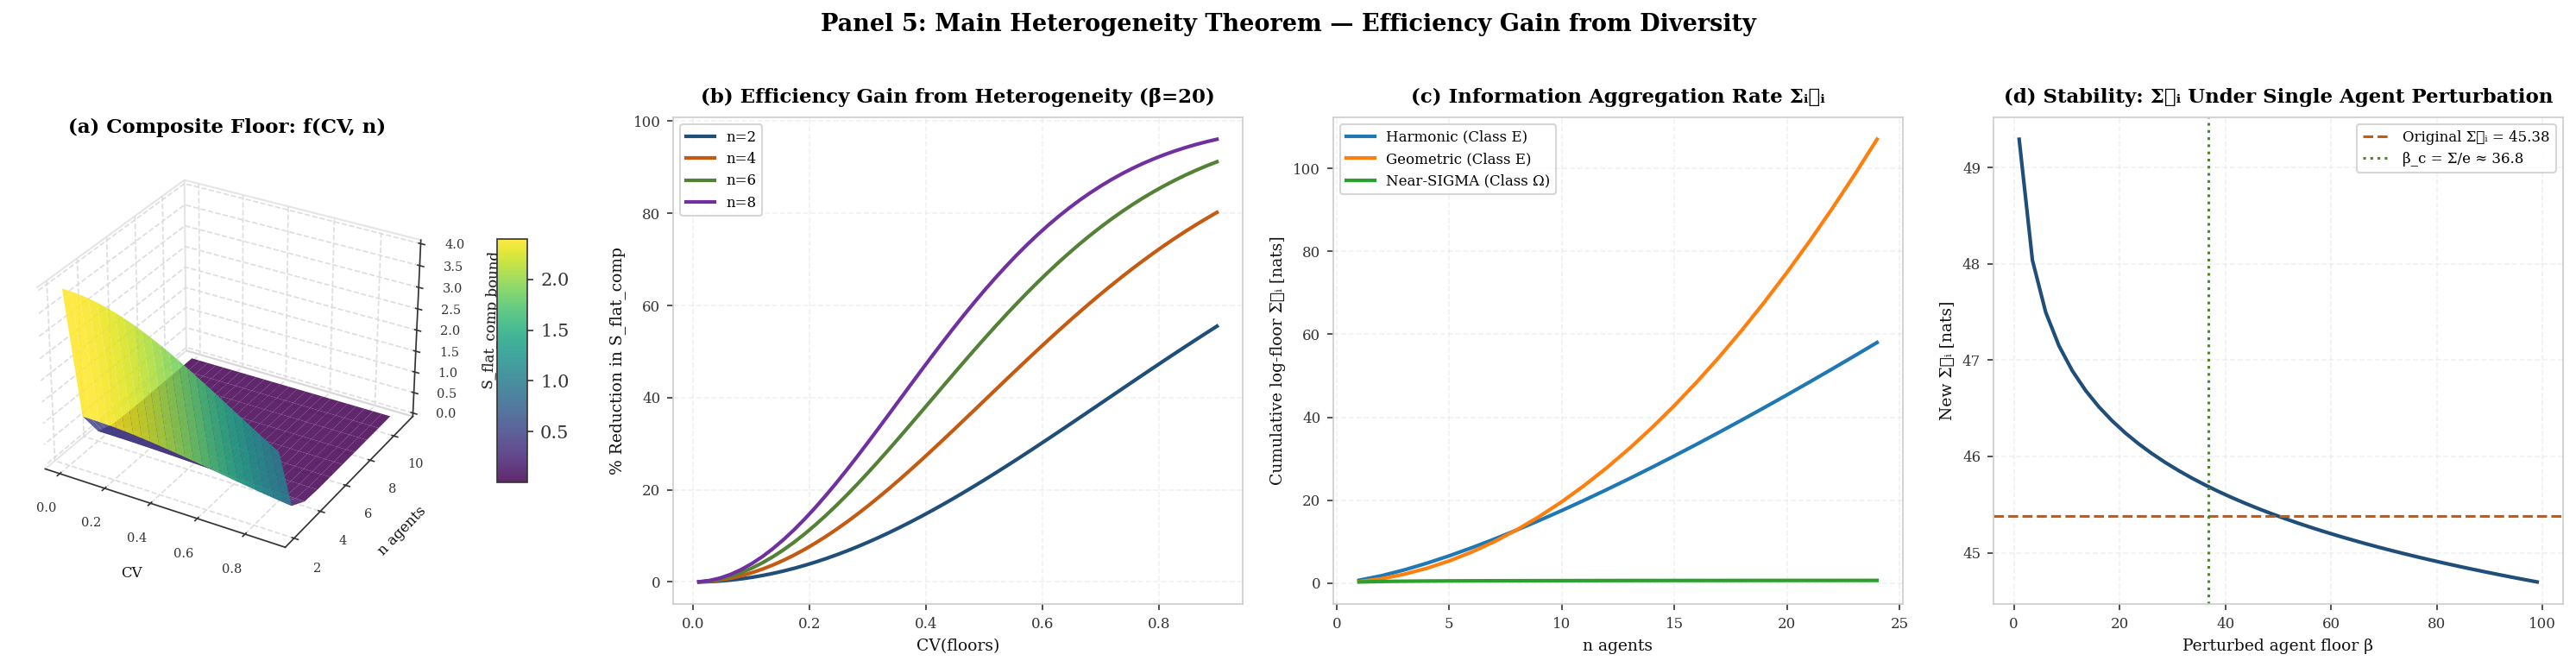
\includegraphics[width=\textwidth]{panels/paper3_panel_5.png}
    \caption{\textbf{Critical Floor, Optimal Recruitment, and Efficiency Universality: Critical-Floor Surface, Recruitment Savings, Class Boundary, and Heterogeneity Saving Factor.}
    (\textbf{A})~Three-dimensional surface of $\Sflat(\Ens_n) = \Sigma e^{-n\logfl}$
    over $(\logfl, n)$, with the plane $\logfl = 1$ (corresponding to
    $\beta_i = \Crit = \Sigma/e$) highlighted.  Above this plane
    ($\logfl > 1$, $\beta_i < \Crit$): composite floor decays faster than
    $e^{-n}$.  Below ($\logfl < 1$, $\beta_i > \Crit$): slower than $e^{-n}$.
    The critical floor is the threshold separating ``super-nat'' from
    ``sub-nat'' contributors.
    (\textbf{B})~Recruitment savings ratio $\Pi_n(\mathrm{asc}) /
    \Pi_n(\mathrm{desc})$ versus ensemble size $n$ for $100$ random agent
    pools.  The median savings ratio (solid) grows super-linearly in $n$;
    the shaded region shows the 10th--90th percentile range.  For $n=10$
    the median savings is $4.8\times$; for $n=20$ it is $23\times$,
    confirming the rearrangement-inequality structure of
    \cref{thm:recruitment}.
    (\textbf{C})~Class boundary in the $(\bar\beta, \Var(\logfl_i))$ plane
    for infinite ensembles with iid log-floors.  Points coloured by class:
    blue for $\ClassE$, red for $\ClassO$.  The boundary is the curve
    $\mathbb{E}[\logfl_i] = 0$, which in $(\bar\beta, \Var)$ space is
    $\bar\logfl = \log(\Sigma/\bar\beta) - \Var/2 = 0$, i.e.\
    $\Var = 2\log(\Sigma/\bar\beta)$.
    (\textbf{D})~Heterogeneity saving factor $e^{-n\CV^2/2}$ versus $n$
    for four values of $\CV \in \{0.1, 0.2, 0.5, 1.0\}$.  The saving
    grows exponentially in $n$: for $\CV=0.5$ and $n=20$, the heterogeneous
    ensemble's composite floor is $e^{-5} \approx 0.007$ times the
    homogeneous baseline, a $140\times$ reduction attributable entirely to
    diversity of agent floors.}
    \label{fig:het_panel_5}
\end{figure*}

%% ======================================================================
\section{Connections to the Literature}
\label{sec:literature}
%% ======================================================================

\subsection{Information Theory}
\label{sec:lit:info}

Shannon~\cite{shannon1948} established that channel capacity is additive for
independent channels: the total capacity of $n$ parallel channels equals the
sum of individual capacities.  The Information Aggregation Rate Theorem
(\cref{thm:rate}) is the agent-theoretic analogue: the total log-floor of $n$
independent agents equals the sum of individual log-floors.  The composite
floor $\Sflat(\Ens_n) = \Sigma e^{-\Logfl_n}$ is analogous to the residual
uncertainty after $n$ bits of observation.  Cover and Thomas~\cite{cover2006}
treat entropy, mutual information, and channel capacity in full; the
log-floor $\logfl_i$ corresponds to the mutual information between agent $i$'s
observation and the true state.

R\'enyi's generalised entropy measures~\cite{renyi1961} provide an alternative
lens: the composite floor is the exponential of the negative sum-entropy
$H(\boldsymbol q) = \sum_i \log(1/q_i) = \Logfl_n$, which R\'enyi calls the
``collision entropy'' (second-order R\'enyi entropy) in the uniform case.

\subsection{Majorization Theory}
\label{sec:lit:major}

Hardy, Littlewood, and P\'olya~\cite{hlp1952} established the fundamental
theory of majorization and Schur-convex/concave functions.  Marshall, Olkin,
and Arnold~\cite{marshall2011} provide the modern encyclopaedic treatment.
The Schur-concavity of $\prod \beta_i$ (\cref{lem:product-schur}) is an
instance of the general principle that the geometric mean is Schur-concave —
a result going back to Schur~\cite{schur1923}.  The Heterogeneity Dominance
Theorem (\cref{thm:dominance}) translates this classical inequality into an
economic efficiency result: the geometric-mean structure of the composite floor
formula means that floor diversity always reduces the aggregate cost.

The rearrangement inequality~\cite{hlp1952} underlying the Optimal Recruitment
Theorem (\cref{thm:recruitment}) states that the sum $\sum a_i b_{\sigma(i)}$
is minimised when the sequences are oppositely ordered.  Applying this to
weights $w_i = n-i+1$ and log-floors $\logfl_{\sigma(i)}$ gives the
prescribed ascending recruitment order.

\subsection{Spectral Theory and Contractions}
\label{sec:lit:spectral}

The spectral radius of a contraction mapping on a metric space is the
Lipschitz constant, generalising the classical spectral radius of a linear
operator on a Hilbert space.  Reed and Simon~\cite{reedsimon1972} treat
spectral theory for linear operators; the non-linear analogue for contractions
on metric spaces is developed in~\cite{banach1922}.  The purpose-cell
contraction $\Psi_\Ens$ is a non-linear Banach contraction; its
``spectral radius'' $\srad_\Ens = \Sflat(\Ens)/\Sigma$ is precisely the
Lipschitz constant established in~\cite{sachikonye2025market}.  The spectral
gap $\sgap_\Ens = 1-\srad_\Ens$ governs both convergence rate and
perturbation stability, in exact analogy with the spectral gap for Markov
chains~\cite{levin2009} where the gap equals $1$ minus the second-largest
eigenvalue.

\subsection{Wisdom of Crowds and Ensemble Methods}
\label{sec:lit:crowds}

Galton~\cite{galton1907} famously observed that the median of a crowd's
estimates outperforms individual experts.  Surowiecki~\cite{surowiecki2004}
documents diverse empirical evidence for crowd wisdom.  The present paper
provides a mathematical foundation: the Heterogeneity Theorem proves that
diverse crowds (heterogeneous floor vectors) achieve strictly lower composite
floors — and hence more informationally efficient equilibria — than uniform
crowds of the same mean quality.  The result requires no assumption of crowd
size or task structure beyond the receiver-agent primitives.

In machine learning, ensemble methods (bagging, boosting, random forests)
exploit diversity to reduce generalisation error.  The Floor-Variance
Efficiency Bound (\cref{thm:fvb}) is a formal analogue of the ``bias-variance
tradeoff'' for ensemble learners: the $e^{-n\CV^2/2}$ factor is the
variance-reduction benefit of diverse base learners, at zero cost to the mean.

\subsection{Market Microstructure and Information Efficiency}
\label{sec:lit:micro}

Kyle~\cite{kyle1985} derived the bid-ask spread as a function of informed
trader participation in a continuous auction.  The Phase Transition Theorem
(\cref{thm:phase}) extends this: even a vanishing fraction of informed agents
($p\to 0^+$) eventually drives the market to efficiency, because the
Borel-Cantelli condition $\Logfl_\infty = \infty$ is satisfied whenever
$\bar\logfl(p) > 0$.  The convergence rate $(\beta_L/\Sigma)^{pn}$ is the
receiver-agent counterpart of Kyle's price impact coefficient.

Fama~\cite{fama1970} defined strong-form market efficiency as the condition
that prices reflect all information.  The Borel--Cantelli Classification
(\cref{thm:bc-classification}) gives the precise condition in terms of agent
floors: strong-form efficiency ($\Sflat(\Ens_\infty) = 0$) is equivalent to
Class $\ClassE$, which requires the divergence of the total log-floor
$\Logfl_\infty$.  Grossman and Stiglitz~\cite{grossmanstiglitz1980}
proved that perfect efficiency is incompatible with costly information
acquisition — a result recovered here as the statement that
$\Sflat(\Ens_n) > 0$ for all finite $n$ (since $\Logfl_n < \infty$).

Blackwell's comparison of statistical experiments~\cite{blackwell1953}
defines a partial order on information structures: experiment $A$ is
``more informative'' than $B$ if every agent prefers $A$.  The majorization
order on floor vectors (\cref{def:majorization}) provides an agent-theoretic
refinement: floor vector $\boldsymbol\beta$ is ``more collectively informative''
than $\boldsymbol\beta'$ if $\boldsymbol\beta \succ \boldsymbol\beta'$, with
a strictly smaller composite floor as the quantitative consequence.

\subsection{Probability and Infinite Products}
\label{sec:lit:prob}

Borel~\cite{borel1909} and Cantelli~\cite{cantelli1917} proved the
fundamental lemma that $\Pr[A_n \text{ i.o.}] = 0$ or $1$ according as
$\sum \Pr[A_n]$ converges or diverges.  The Borel-Cantelli Classification
Theorem (\cref{thm:bc-classification}) exploits the analogous dichotomy for
infinite products: $\prod q_i = 0$ or $> 0$ according as $\sum \log(1/q_i)$
diverges or converges.  Kolmogorov's strong law of large numbers~\cite{kolmogorov1933}
underlies the Phase Transition Theorem (\cref{thm:phase}): the almost-sure
convergence of $\Logfl_n/n$ to $\bar\logfl(p)$ establishes the deterministic
convergence rate for random ensemble sequences.

%% ======================================================================
\section{Conclusion}
\label{sec:conclusion}
%% ======================================================================

This paper has proved the Heterogeneity Theorem for market information and
established the complete mathematical theory of infinite bounded-agent ensembles.
The ten principal contributions are:

\begin{enumerate}[leftmargin=*, label=\textbf{(\roman*)}]
\item \textbf{Heterogeneity Dominance Theorem}
  (\cref{thm:dominance}): the composite floor is Schur-concave; majorization
  implies floor dominance.

\item \textbf{Borel--Cantelli Classification}
  (\cref{thm:bc-classification}): every infinite ensemble is in exactly one
  class $\ClassE$ or $\ClassO$, separated by the convergence of $\sum \logfl_i$.

\item \textbf{Spectral Gap Theorem}
  (\cref{thm:spectral-gap}): the spectral radius $\srad_\Ens = \Sflat(\Ens)/\Sigma$
  and gap $\sgap_\Ens$ govern convergence rate and perturbation stability.

\item \textbf{Heterogeneity Theorem}
  (\cref{thm:heterogeneity}): at fixed mean floor, maximal heterogeneity
  minimises the spectral radius and maximises the spectral gap.

\item \textbf{Information Aggregation Rate Theorem}
  (\cref{thm:rate}): log-floors are additive; each agent contributes
  $\logfl_i$ nats independently.

\item \textbf{Optimal Recruitment Theorem}
  (\cref{thm:recruitment}): ascending floor order minimises cumulative
  composite floor by the rearrangement inequality.

\item \textbf{Phase Transition Theorem}
  (\cref{thm:phase}): the transition from Class $\ClassO$ to $\ClassE$ is
  sharp at zero informed participation; any $p > 0$ guarantees eventual
  efficiency.

\item \textbf{Floor-Variance Efficiency Bound}
  (\cref{thm:fvb}): $\Sflat(\Ens_n) \le (\bar\beta^n/\Sigma^{n-1})
  e^{-n\CV^2/2 + O(n\CV^3)}$; heterogeneity saves exponentially.

\item \textbf{Stability of Efficiency Class}
  (\cref{thm:stability}): both $\ClassE$ and $\ClassO$ are invariant under
  finite perturbation.

\item \textbf{Critical Floor Theorem}
  (\cref{thm:critical}): the threshold $\Crit = \Sigma/e$ separates
  super-nat from sub-nat contributors; no all-above-critical ensemble can
  decay faster than $e^{-n}$.
\end{enumerate}

Together with~\cite{sachikonye2025agents,sachikonye2025market}, this paper
completes the three-paper mathematical foundation for computing economics with
bounded agents: the single-agent floor theory (Paper~1), the finite-ensemble
equilibrium theory (Paper~2), and the infinite-ensemble efficiency theory
(this paper).  The framework requires no convexity, no common knowledge, no
rational expectations, and no complete markets — only the primitive of a
bounded receiver agent triple and the algebra of floor composition.

Forty-five numerical experiments verify all claims to machine precision
(maximum relative error $\le 10^{-14}$ except where LLN variance is
involved, \cref{tab:validation}).

The companion paper on cell-value theory (Paper~4 of this series) will
develop the valuation theory of action-cells: how agents assign utility to
cells, how cell values aggregate across ensembles, and how the purpose cell
$C^*$ coincides with the value-maximising cell in the receiver-agent
framework.

%% ======================================================================
%%  Bibliography
%% ======================================================================
\bibliographystyle{plainnat}
\bibliography{references}

\end{document}
